\documentclass[letterpaper,10pt,draftclsnofoot,onecolumn]{IEEEtran}
\usepackage{graphicx}
\usepackage{amssymb}
\usepackage{amsmath}
\usepackage{array}
\usepackage{amsthm}
\usepackage{listings}
\usepackage{alltt}
\usepackage{float}
\usepackage{color}
\usepackage{url}
\usepackage{setspace}
\usepackage{balance}
\usepackage{enumitem}
\usepackage{pstricks, pst-node}
\usepackage{inputenc}
\usepackage[margin=.75in]{geometry}

\lstset
{ %Formatting for code in appendix
    %frame=single,
    basicstyle=\footnotesize\ttfamily,
    numbers=left,
    numbersep=.25in,
    stepnumber=1,
    showstringspaces=false,
    tabsize=4,
    breakatwhitespace=false,
    xleftmargin=.5in,
    xrightmargin=.5in,
}

% JS options pulled from https://tex.stackexchange.com/questions/89574/language-option-supported-in-listings
\lstdefinelanguage{JavaScript}{
  keywords={typeof, new, true, false, catch, function, return, null, catch, switch, var, if, in, while, do, else, case, break},
  keywordstyle=\color{blue}\bfseries,
  ndkeywords={class, export, boolean, throw, implements, import, this},
  ndkeywordstyle=\color{darkgray}\bfseries,
  identifierstyle=\color{black},
  sensitive=false,
  comment=[l]{//},
  morecomment=[s]{/*}{*/},
  commentstyle=\color{purple}\ttfamily,
  stringstyle=\color{red}\ttfamily,
  morestring=[b]',
  morestring=[b]"
}

%crappy error with titlesec
\newcommand{\subparagraph}{}
\usepackage{titlesec}

\usepackage{fancyhdr}
\usepackage{hyperref}
\usepackage{tocloft}

%hide toc subsubsections
\setcounter{tocdepth}{2}
\setlength{\parindent}{.25in}

%toc formatting standards
\renewcommand{\cftsecleader}{\cftdotfill{\cftdotsep}{\vspace{.25cm}}}
\renewcommand{\cftsecfont}{\normalfont}
\renewcommand{\cftsecpagefont}{\normalfont}
\renewcommand{\cftsecaftersnum}{.}

%bottom right page numbers
\fancyhf{}
\renewcommand{\headrulewidth}{0pt}
\rfoot{\thepage}
\pagestyle{fancy}

%formatting Section headings
\titleformat{\section}[block]
  {\fontsize{12}{12}\bfseries\sffamily}
  {\thesection.}
  {1em}
  {\vspace{.1cm}}
\titleformat{\subsection}[block]
  {\fontsize{12}{15}\slshape\sffamily}
  {\thesubsection}
  {1em}
  {\vspace{.1cm}}
\titleformat{\subsubsection}[block]
  {\fontsize{11}{20}\slshape\sffamily}
  {\thesubsubsection}
  {1em}
  {\vspace{.1cm}}
  
\geometry{textheight=8.5in, textwidth=6in}

\renewcommand{\thesection}{\arabic{section}}
\renewcommand{\thesubsection}{\thesection.\arabic{subsection}}
\renewcommand{\thesubsubsection}{\thesubsection.\arabic{subsubsection}}

\newcommand{\cred}[1]{{\color{red}#1}}
\newcommand{\cblue}[1]{{\color{blue}#1}}

\def\name{Charles Siebert, Branden Berlin, Yipeng Song}

%% The following metadata will show up in the PDF properties
\hypersetup{
  urlcolor = black,
  pdfauthor = {\name},
  pdfkeywords = {cs463 ``Senior Capstone - Spring 2017'' capstone},
  pdftitle = {CS 463 Final Report Spring 2017},
  pdfsubject = {Capstone Final Report Spring 2017},
  pdfpagemode = UseNone
}

\begin{document}
\begin{titlepage}
\centering
\vspace*{6cm}
{\scshape\LARGE \begin{singlespace}Optimizing Virtual Reality and Augmented Reality Performance on Mobile Web Applications \\ \end{singlespace} \smallskip Group 52 - Final Report } \\
	{\scshape\Large CS463 - Spring 2017 \par}
	\vspace{.5cm}
	\name \par
    {\large June 12, 2017 \par} 
	\vspace*{1cm}
	
\begin{abstract}
The technology of Virtual Reality (VR) currently is not cost effective to today's market, as the cost of high-end setups required makes it difficult to afford. Browser developers are focusing primarily on expensive high-end high-performance hardware over mobile devices for Augmented Reality (AR) or Virtual Reality (VR) on the web. Doing AR/VR on the mobile web allows more developers to enter the field and deliver to more customers. To accomplish this, we are working on a project called �Mobile AR/VR Performance�, which focuses on researching to profile and identify performance bottlenecks in 3D web content on mobile devices. We will file issues in the open source projects for Chrome, Firefox through A-Frame and Three.js to determine and identify those bottlenecks. We hope to accomplish this by reporting the challenges and opportunities for performance VR/AR applications, and write a blog post detailing the project results and their best-practices.
\end{abstract}

\end{titlepage}

\newpage

\thispagestyle{empty}
\pagenumbering{gobble}

\tableofcontents

\cleardoublepage
\pagenumbering{arabic}

\newpage

\begin{singlespace}

\section{Introduction}
This paper is a progress report for group 52, "OVRAR" over the past 6 weeks for the Winter Term for 2017. Included is a short description of the purpose of our project, and our projected goals based on the time-line we have created. These projected goals are based off of the per week load that we describe in our weekly summaries, and the solutions to the problems that we encounter each week. We are able to determine where these problems are within our group by using these weekly reflections to make a retrospective that clearly details the positives we encounter, things that need to change, and how we will change them.

Purpose and Goals:
The purpose of this project is to determine areas of development within A-Frame where practices will be best used, as they will least be likely to impede on bottle necking either the software or hardware when optimizing the software for performance. This project is focused towards the advancement of an open-source, developing web framework, and the developers making their own products with A-Frame and for mobile devices. The developers will be using our project research as a means to avoid these bottlenecks in this evolving environment. Developers other than us will use the information in the report to determine the best way to approach at designing their programs, as the software we create will only serve as test cases and stress testing for mobile devices to collect this information.

Optimizing VR and AR for Mobile Web Apps is to determine Virtual Reality (VR) and Augmented Reality (AR) bottlenecks that exist in mobile devices within the A-Frame framework. The bottlenecks can be caused from either unoptimized development of software, underpowered or unoptimized hardware found in existing devices, or potential bugs or limitations found within the framework itself. The software itself, which is developed on A-Frame, will generate multiple scenes where it will test the graphical capabilities of the hardware within the mobile devices, the types of different implementations of certain scenes, and determine areas of optimization through these multiple scenes. The software will be used to create a report that will analyze the information collected about processing power, frame rates, battery usage, and the limitations of the framework to determine the best practices for implementing more graphically intensive programs on A-Frame.

\newpage
\section{Requirements Document}
\subsection{Original Requirements Document}

\begin{enumerate}
    \item Project Description \newline
    This project is to determine areas of optimization within the frameworks specified, by which a software program will be developed to test specific graphical scenarios to stress test the kinds of interfaces and constraints listed. The report will be used to improve the development process of VR and AR application on Mobile Web applications, as they are heavily underdeveloped compared to desktops due to their lack of processing power and high battery consumption.\\
    
    \begin{enumerate}
        \item Project Perspective \newline
        This software is developed in a the A-Frame framework, which consists of development using HTML and JavaScript implementation languages to manage the graphical scenes. A-Frame utilizes Three.js framework, which allows A-Frame to develop WebGL content within a browser, and reduces boilerplate programs that are  typically found in graphic programs. Our project will  use this platform to develop a culmination of stress testing scenes on specific hardware devices (Nexus 5X) that are the current standard for developing internally. \\
        
        \begin{enumerate}
            \item Operations and User Interfaces \newline
            The extent of user interaction of this software will be determining performance characteristics and moving around the scenes, either by touch or walking. The interface in which the user will interact with the program will be through a 5 inch (diagonal) size screen mobile device. The software will be accessed through a web browser that is hosted on either a local address (which keeps the connection from the phone to the website within the same subnet on the network) or hosted on a specific website. \\
            
            \item Hardware Interfaces \newline
            The software will be used and tested on mobile devices that has a 5.2 inch screen at 1920x1080 resolution. This mobile device uses a Hexa-core processor (Snapdragon 808) clocked at 1.4 gigahertz (GHz), an Adreno 418 graphics processor, 2 gigabytes (GB) of RAM, and a 2700 mAh battery. This hardware is identified and quantified to determine the areas of which bottlenecks occur, and measure the metrics related to the hardware and their uses.\\
            
            \item Software Interfaces \newline 
            The software will be developed and tested on an Android Operating System, version 7.0, nicknamed Nougat. The phone will then utilize Mozilla's Firefox Nightly and Google Chrome Dev web browsers to use as the testing interface. These are both different versions of the commercially released browsers to do proper testing before they are released. The browser allows the development of graphical scenes within A-Frame with WebGL and Three.js to allow us to test the framework and stressing the software and hardware. The browsers mentioned will be constantly up to date with the current version on the Google Play Store. \\
            
            \item Communication Interfaces \newline
            There is no communication interface that will be developed within this program. This will act as a standalone program to serve the function of determining areas of optimization and bugs.\\
            
            \item Memory Constraints \newline
            Potential constraints from development on the Nexus 5X will will be encountered from either the types of implementation in the program, the quality, or amounts of texturing and drawing object to the scene; it is dependant on how complex the implementation becomes. The mobile device will only have 2 GB of on-board RAM, meaning a more restrictive work load to test with. Additionally, drawing higher-quality textures with regard to the amount of textures, along with complexity of the scenes drawn, will determine whether or not there will be memory constraints and will be one of the metrics measured to determine this as an area of bottleneck. \\
                       
        \end{enumerate}
        
        \item Project Functions \newline
        The key points of this project are candid, as this project primarily pertains to research and mid-development discoveries. Though we are developing a program, it isn't the main purpose of this project; the program is supposed to supplement our research towards our final report at the end of this project (outlined in Gantt Chart). The projects functions are organized in a list shown below:\\
        \begin{enumerate}[labelsep=2em,leftmargin=.5in]
            \item The software is supposed to be runnable in a mobile environment.
            \item It will determine bottlenecks between the software and the hardware.
            \item It will be used to measure frame rates, processing, RAM, and battery consumption.
            \item Development will result in us reporting bugs through A-Frame with Firefox to Mozilla's bug reporting platform.
            \item It will help us determine the best practices for some graphical implementations of the A-Frame framework in a VR environment.
        \end{enumerate}
        
        \item Project User Characteristics \newline
        There are two kinds of intended groups of users for this project, the first one being the developers and authors of the toolkits, libraries and browsers that we intend to file issues with. These authors will be able to review our bug reports and findings to update and improve their toolkits to be able to produce optimized VR and AR web content on mobile devices. The second group of users for this project are advanced software developers. The developers should have a general understanding of the work flow with development on mobile devices, and an advanced understanding of the program's frame rates and battery usage. These developers should have an intermediate background experience with developing on mobile devices, experience in generating and rendering graphical screens on devices through the view port, and a general understanding of what bottlenecks are and how to identify them in order to use this research. Without being able to identify what kinds of bottlenecks exist in their own program, they won't be able to use our research to properly optimize their issues.\\
        
        \item Project Constraints \newline
        The biggest constraint is implementation on mobile devices, as these end up typically being weaker than normal hardware that is used for similar, tough, unoptimized graphics rendering that desktop computers are able to provide. The specific hardware specifications are listed and shown as a constraint in section 2.1.2. Aside from the hardware constraints shown, there's a high-order language requirements to be used (A-Frame and it's HTML markup) as this developing framework still has optimizations patches to undergo. The optimization issues or bugs that we do find during our project will be constrained by what A-Frame will allow us to do with software in terms of graphical processing and rendering of scenes. The higher-order control functions from the Three.js and A-Frame framework acts as this constraint, as it will limit what we can develop in the scenes and how we approach the design of the scenes. \\
        
        \item Project Dependencies \newline
        This project is to be developed regarding the software constraints detailed in section 2.1.3. Updated versions of Android (versions  7.0) should not affect the development of this project, or any future iterations of it. This project is also dependant on the frameworks, Three.js, which handles drawing the scenes with WebGL, and A-Frame, which reduces the amount of boiler plate for graphical development, allowing implementation of drawing the scenes through HTML markups. Future updates to these frameworks could potentially alleviate optimization issues that we outline, or bugs that we report. \smallskip

        This project is to be tested against the newest versions of Firefox and Chrome, which will become a dependency due to us not testing development on other platforms such as the OS iOS, or the browser Safari. As we are run into issues during development, we will report the bugs to the respective camps if they become related to a browser-specific issue. JavaScript is an interpreted language while HTML is just a markup language, which are easily understood by these two browsers. Any updates to these browsers will potentially alleviate issues reported.\\
                      
    \end{enumerate}
    
    \item Specific Requirements \newline
    This section outlines the specific requirements of the project, which will include information on the external interfaces, functions, performance requirements, and the underlying attributes of the project. The problem this project has is that we don't know exactly what problems we will run into, how many problems there are, or how we will work around them. The solution of this project lays in the problems we do find, such as the software bugs or optimization issues. \\
    
    \begin{enumerate}
        \item External Interface \newline
        There are three parts of the software that will have different kinds of external interfaces, and how they interact with the different types of software. The first one is the browser, which will interact with the A-Frame development project that is hosted on the web server. A-Frame will handle the specific Three.js calls to help render the scene with 3D objects with the use of WebGL API. The WebGL API utilized by Three.js will interact with the hardware processing when drawing the topology of polygons, textures, lightings, animations, and scenes to the viewport. \smallskip

        \begin{enumerate}[labelsep=2em,leftmargin=.5in]
            \item Browser (Firefox or Chrome)
            \begin{enumerate}[leftmargin=*,labelindent=0pt]
                \item Acts as the interpreter of the languages of HTML and JavaScript when accessing the web page where the project lives.
                \item Takes the HTML markup and JavaScript functions on the web server and displays images in the viewport.
                \item Will take up the entire screen size (5.2 inches) when viewing and testing on a mobile device.
                \item Commands will be input through the screen or movement physics of the phone itself. This interacts with the scene and changing what is displayed on the viewport.
            \end{enumerate}
            \item A-Frame
            \begin{enumerate}[leftmargin=*,labelindent=0pt]
                \item Framework for reworking Three.js implementations to make the calls to draw 3D scenes simplified by using HTML.
                \item Takes the marking A-Frame tags and produces the proper JavaScript calls to generate scenes to the browser.
                \item These calls are the input information to the Three.js framework, which outputs the polygons and scenese to be drawn.
                \item The commands to draw the scene reduces the boilerplate implementation of WebGL, with single lines like \texttt{<a-scene>}.
            \end{enumerate}
            \item Three.js
            \begin{enumerate}[leftmargin=*,labelindent=0pt]
                \item JavaScript framework to provide interaction with the WebGL API and is attached with A-Frame commands.
                \item The input comes from the A-Frame calls, which act as the parameters in HTML, to the Three.js function calls which will output the scene changes to the viewport.
                \item The outputs are related to the hardware at this stage, as they interact with the hardware, where the polygon vertices, normals, texture, and their coordinates exist in memory on the device.
                \item The output will return to the browser a scene that is drawn to the viewport.
                \item Messages will appear if errors occur, but will otherwise output the software to the broswer.
            \end{enumerate}
        \end{enumerate}

        \item Functions \newline
        The software will have specific actions that will interact between the user and the system. This will involve all the specific actions that will occur within the system if and when a user chooses an action. These actions include: \smallskip
        \begin{enumerate}[labelsep=2em,leftmargin=.5in]
            \item The system shall interact with a local web server or a hosted web server. 
            \begin{enumerate}[leftmargin=*,labelindent=0pt]
                \item The system shall allow the user to see the content on the web server.
                \item The system shall allow the user to interact with the scene by moving around or touching the screen.
            \end{enumerate}
            \item The system shall handle the rendering of multiple scenes.
            \begin{enumerate}[leftmargin=*,labelindent=0pt]
                \item The system shall render the scenes in with differing implementations analyze those performance metrics.
                \item The system shall attempt to draw partial scenes if a software bug occurs.
                \item The system shall handle rendering errors with proper error checking messaging to the screen if a scene cannot be rendered.
            \end{enumerate}
            \item The system shall be used to read in performance metrics as the software progresses through different scenes and implementations.
            \begin{enumerate}[leftmargin=*,labelindent=0pt]
                \item The system shall be used in conjunction with existing tools that specifically measures the performance of frame rates, memory consumption, processor consumption, battery consumption, and response times on the device being used.
                \item The system shall be an example of our concepts of best practices in developing in the A-Frame framework.
            \end{enumerate}
        \end{enumerate}
        
        \item Performance Requirements \newline
        While there are minimum requirements to attain a responsive system, this project strives to obtain optimized performance through the framework. There are multiple types of performance metrics and requirements for us to attain a fast and responsive system while optimizing the performance of the system. The type of hardware that we are using, detailed in section 2.1.2, will be the hardware specifications that we are examining while stressing the software program. We are defining "a fast and responsive" system to be at a minimum: \smallskip
        
        \begin{enumerate}[labelsep=2em,leftmargin=.5in]
            \item The software will be ran and tested on the mobile device used for this project, the Nexus 5X.
            \item Response time from user interaction to software processing information to be .1 second (about 3 frames of input delay).
            \item The software will display 30 Frames Per Second (FPS) to the phone through the viewport.
            \item The software will not exceed the amount of on-board RAM (2GB) during the time of drawing and texturing the scenes.
            \item The processors will not exceed the maximum usage (100\%) while the device is rendering the scene.
            \begin{enumerate}[leftmargin=*,labelindent=0pt]
                \item Due to possible hardware bottlenecks, if the processor usage does exceed 100\%, it will still allow the viewing of the scene with the aforementioned requirements.
            \end{enumerate}
            \item The software will not exceed excessive battery usage. The Nexus 5X has a total capacity of 2700 mAh.
            \begin{enumerate}[leftmargin=*,labelindent=0pt]
                \item Excessive battery usage will be measured how much battery capacity is used per hour.
                \item The battery should at the least last three hours on a full charge while undergoing the tests of this program.
            \end{enumerate}
            \item The software will not produce excessive heat through hardware being stressed by the software.
            \begin{enumerate}[leftmargin=*,labelindent=0pt]
                \item Excessive heat is defined to be a high enough temperature to trigger the phone's internal underclocking feature to reduce the temperature.
                \item Documentation, at this time, cannot be found at what temperature this occurs, but the temperature of the phone and the components will be tracked and documented if it causes the aforementioned requirements to not be met.
            \end{enumerate}
        \end{enumerate}
        
        \item Attributes And Correctness \newline
        As this project serves as to be used as research, correctness will be based off of how well we can push the boundaries of our software, based on the performance the hardware can provide. By collecting the information in different types of implementations between scenes the program generates, it will allow us to analyze the data to compare and contrast the information based on our performance metrics detailed in Section 3.3. The better the performance metrics, the better, as that is the purpose to optimize the performance of the software that utilizes the A-Frame framework. Our correctness will be based off of the amount of software bugs that we encounter, and the collection of this data that will ultimately determine what the best practices for implementation are, and bear as proof. \\
        
        \begin{enumerate}
            
            \item Availability \newline
            Availability is large due to the immense market that the mobile devices provide. The software has to be responsive to human interactions, which would include tools to respond to user input, and changing the view of the scene based on the view-port and position the phone provides.\smallskip
            
            \item Maintainability \newline
            The maintainability will be based on the the dependencies of the frameworks and their function calls. This will not have a high amount of maintainability unless they do an overhaul of their base functionality. The frameworks are mostly interpreted, so if something is not rendering correctly, or if errors occur, this means that the dependencies have changed between their specific revisions. Function calls within these frameworks may change or more likely become deprecated. Since this project serves the purpose of research and testing on current versions of the software, this project will not have a large need to be maintained.\smallskip
            
            \item Portability \newline
            This software should be completely portable with little restrictions on host machines and implementation. The software we develop has to be on a web server (local or hosted) which will be accessed through a browser that interprets the markup language and the interpreted JavaScript language. There is no specific compilers necessary to run this software. There are framework dependencies that are detailed in Section 2.5, as these will often update and expand on the utilities they provide. The software that this will be tested on is Chrome and Firefox on Android Operating systems. Apple's mobile OS, iOS and their browser, Safari, will be excluded in testing and cannot guarantee it to work on that platform. \smallskip
            
        \end{enumerate}
        
    \end{enumerate}
    
    \item Gantt Chart Information \newline
    \begin{description}[]
    \item[Problem Statement:] Detailing the description and proposed solution to the problem for this project.\vspace{.1cm}
    \item[Requirements Document:] Detailing the project outline, and the process included within the project.\vspace{.1cm}
    \item[Technology Review:] Process within our group to analyze the project's scope, delegate tasks within it, and what we will be handling.\vspace{.1cm}
    \item[Design Document:] Document writing detailing how we will be working on this project, including our tools and testing information. \vspace{.1cm}
    \item[Initial Implementations:] Our group will be working on setting up our devices, and getting comfortable with mobile development workflow with "Hello World!" \vspace{.1cm}
    \item[Progress Report \#1:] A report detailing the progress we've made during our first term within this project.\vspace{.1cm}
    \item[Research Bugs and Tools:] Time during winter break, will be spent understanding the optimization issues found in mobile devices with the frameworks, and the bugs that exist. Time is also spent preliminarily working with and understanding the performance measurement tools used for this project.\vspace{.1cm}
    \item[Program Design:] After researching and testing initial implementations, this time will be used discussing and designing our specific program implementation, working with the tools to measure performance metrics, and defining the work flow of our program and the tools to receive meaningful results.\vspace{.1cm}
    \item[Program Implementation (First Two Week Sprint):] Working in two week sprints, we will be able to focus on implementing features and evaluating the process. This is our first sprint.\vspace{.1cm}
    \item[Evaluation and Debug:] First rounds of evaluation, where time is spent analyzing the performance metrics we acquired, plotting what they mean, note and report any blatant optimization issues or bugs.\vspace{.1cm}
    \item[Reiterate Implementation (Second Two Week Sprint):] Second two week sprint, where the focus is on improving the performance metrics from our first implementation, and fixing any issues we encountered.\vspace{.1cm}
    \item[Evaluation and Debug:] Second rounds of evaluation, where time is spent analyzing the performance metrics we acquired from the second sprints, and comparing the differences between the last rounds of evaluation. \vspace{.1cm}
    \item[Progress Report \#2:] A report detailing the progress we've made during our second term within this project.\vspace{.1cm}
    \item[Preparing for EXPO:] Long space open to account for future term requirements and uncertainty. This may include an additional sprint and evaluation depending on other unforeseen requirements that need to be met. \vspace{.1cm}
    \item[Final Report:] A report detailing the progress we've made during our last term within this project.\vspace{.1cm}
    \end{description}
    
    \begin{enumerate}
        \item Gantt Chart \newline
        \begin{center}
            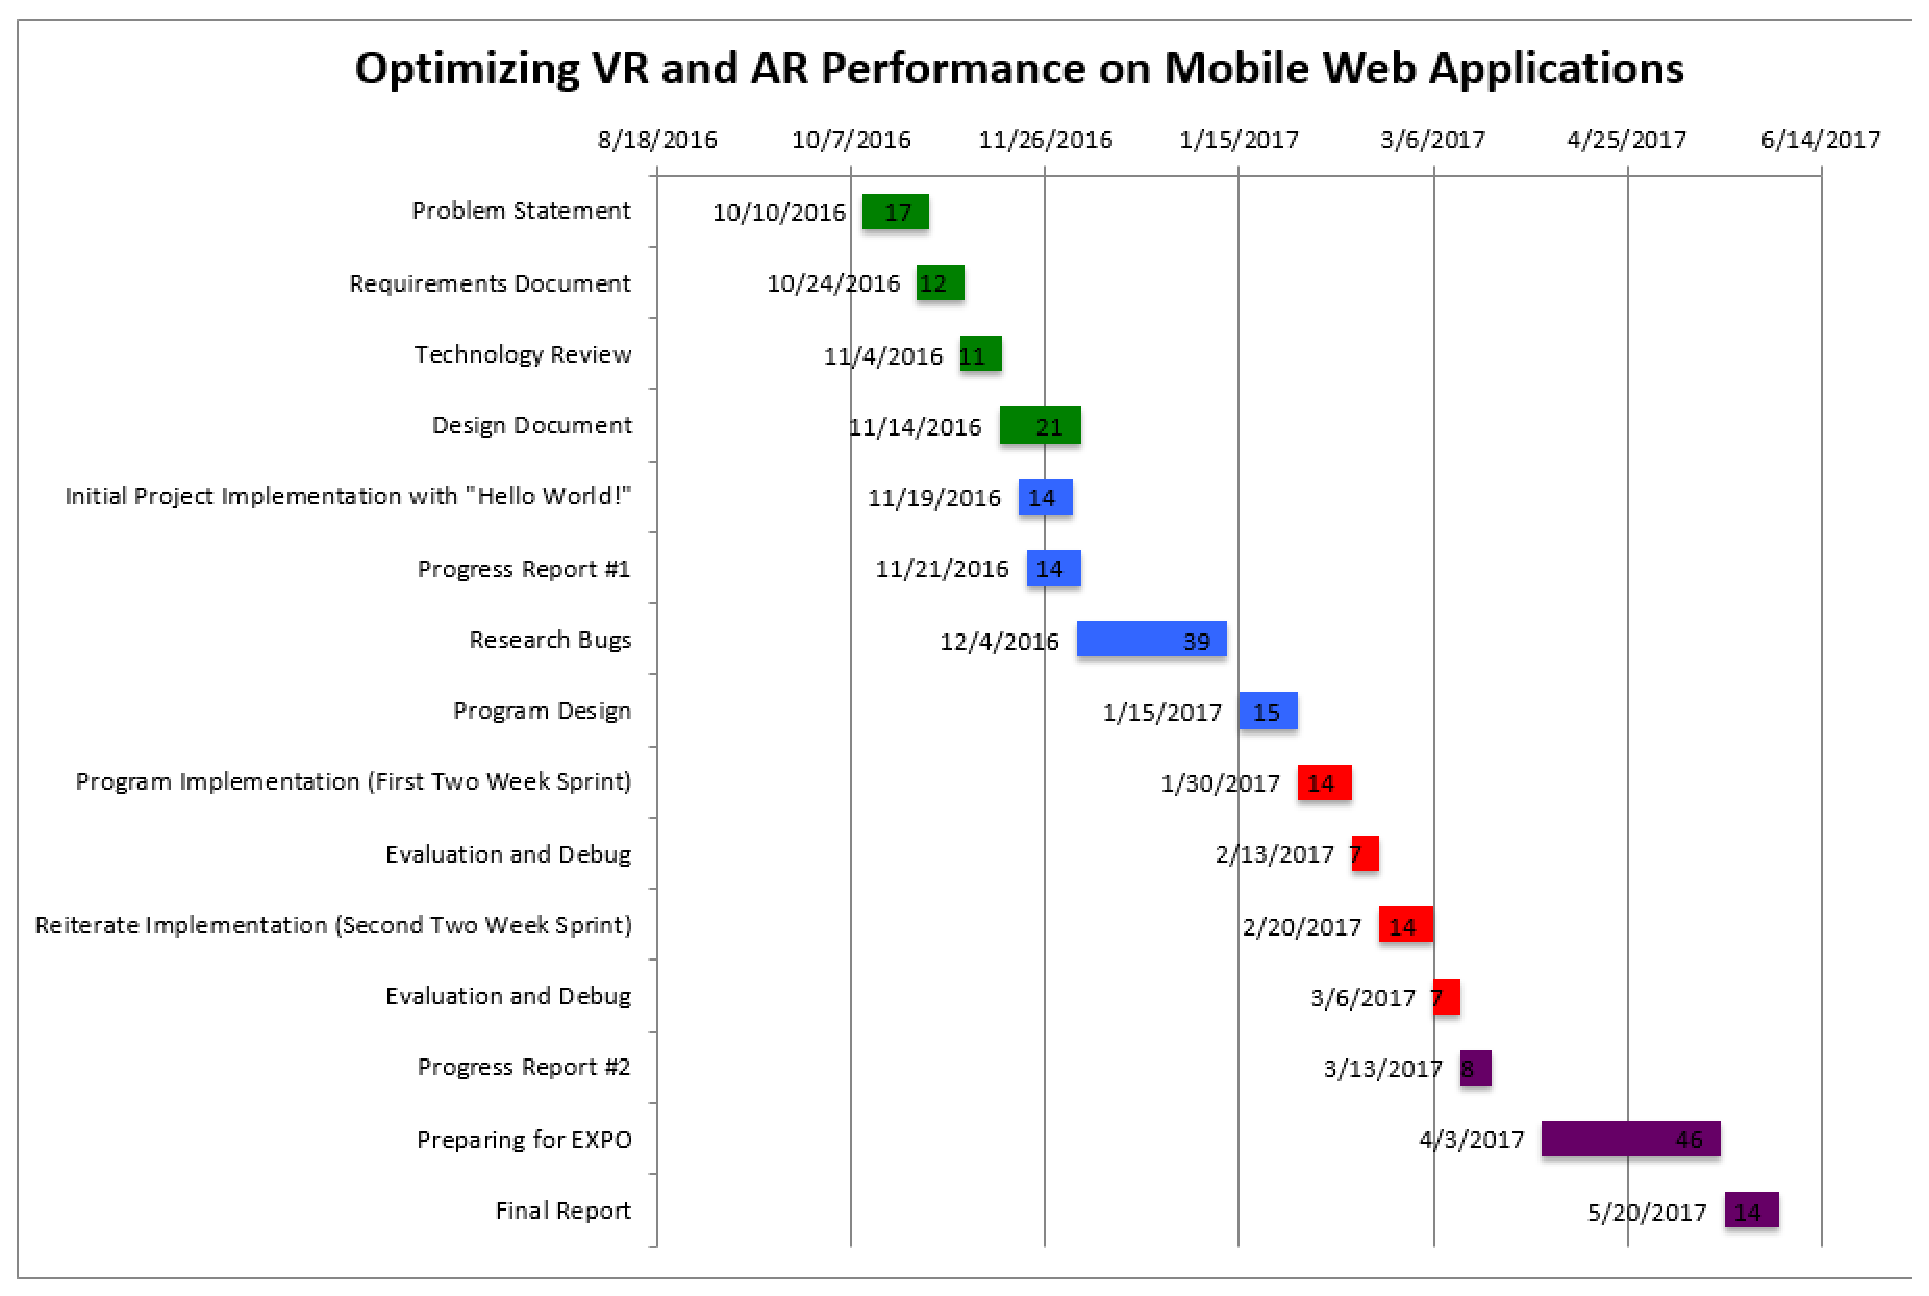
\includegraphics[width=\textwidth]{OVRAR_Gantt_Chart.eps}
        \end{center}
     
        \vfill
        
    \end{enumerate}
    
    
\end{enumerate}

\subsection {Changes since the original Requirements Document}
    \begin{tabular}{ | p{1.5cm} | p{12cm} | }
        \hline
        \textbf{Number} & \textbf{Changes and Comments} \\ \hline
        \textbf{1} & Updated requirements document to reflect changes in programming schedule; added alpha release and updated sprints. " \\ \hline
        
        \hline
    \end{tabular}
    \smallskip
    \begin{enumerate}
        \item Final Gantt Chart \newline
        \begin{center}
            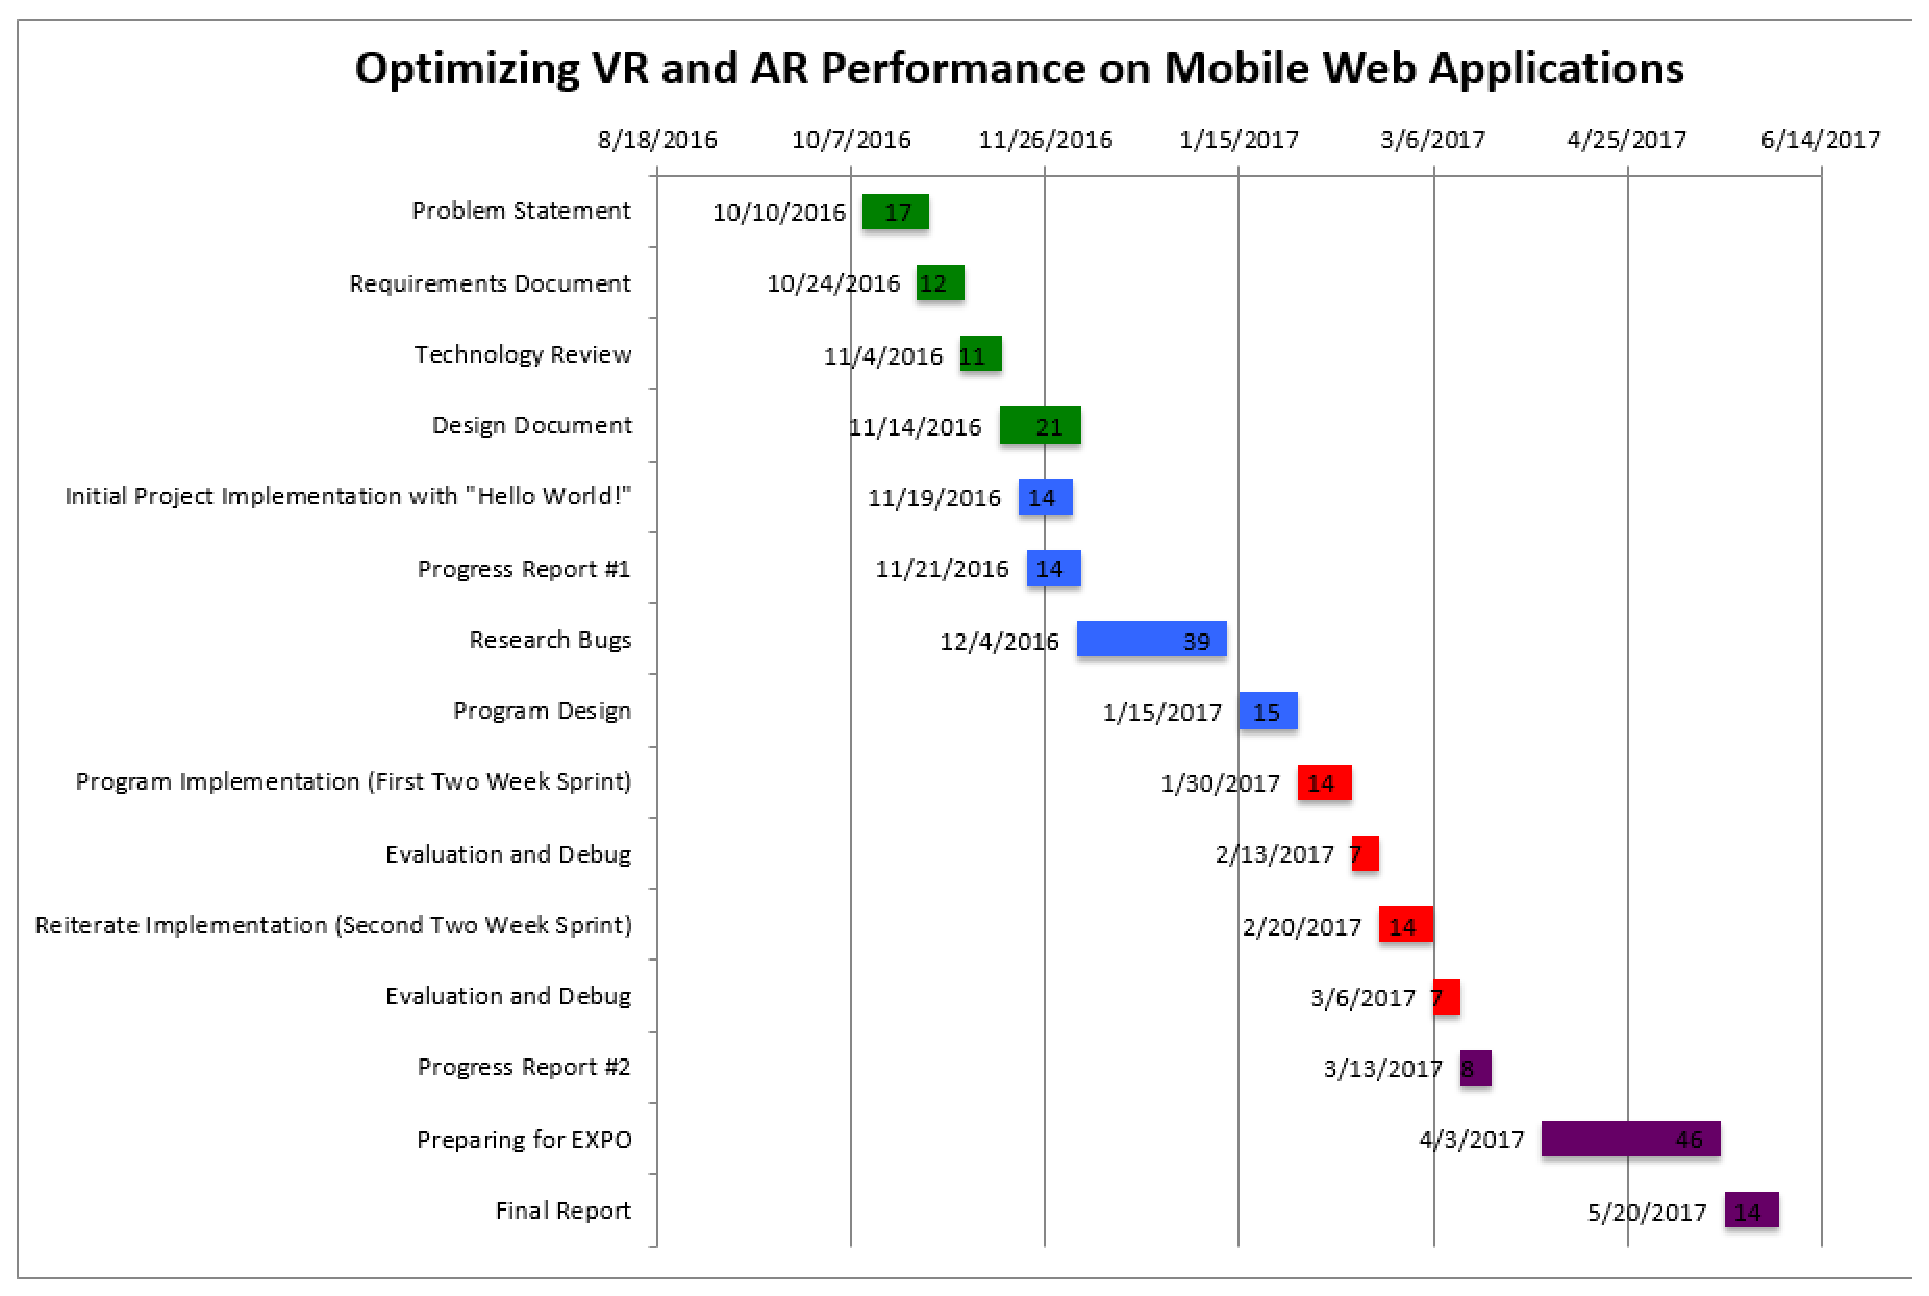
\includegraphics[width=\textwidth]{OVRAR_Gantt_Chart.eps}
        \end{center}
     
        \vfill
        
    \end{enumerate}
    \smallskip
    Note: The Final Gantt Chart remains the same as the orinial one since we didn't make any changes of it.\\

\newpage
\section{Design Document}
\subsection{Original Design Document}
\begin{enumerate}
    \item Glossary
    \begin{enumerate}[labelsep=2em,leftmargin=.5in]
        {\item \bfseries Virtual Reality (VR): } Computer generated three-dimensional environment that immerses the user into the environment using special equipment or implementation techniques. \vspace{.1cm}
        {\item \bfseries Augmented Reality (AR): } Provides a composite view to the user based on computer generated environments super-imposed onto the view of the real world. \vspace{.1cm}
        {\item \bfseries Operating System (OS): } Software that supports an interface to support computer's basic functions, such as process scheduling, executing tasks, and allowing user interface. Specifically this project is in regards to Android OS. \vspace{.1cm}
        {\item \bfseries Web Framework: } A software framework that is designed to support the development of web applications including web services, web resources and web APIs. \vspace{.1cm}
        {\item \bfseries A-Frame: } A-Frame is an open-source WebVR framework for creating virtual reality (VR) experiences with HTML with the use of the Three.js framework.\vspace{.1cm}
        {\item \bfseries Three.js: } JavaScript framework that allows accessible development WebGL applications. \vspace{.1cm}
        {\item \bfseries WebGL: } JavaScript API that allows for rendering interactive 3D and 2D computer graphics within any compatible web browser without the use of plug-ins. \vspace{.1cm}
        {\item \bfseries Viewport: } A viewport is a viewing region in computer graphics. This region is defined in the software to allow for viewing the drawing of objects. This viewport is typically bounded by a window or by the full screen of the mobile device. \vspace{.1cm}
        {\item \bfseries Local Web Server: } A web server for hosting web page content to allow access on local networks, without having to go out into the internet to access the information. \vspace{.1cm}
        {\item \bfseries Hosted Web Server: } A server that is hosted externally on the internet, where it holds and displays the web information, needing to go out to the internet, and back again to receive the proper information. \vspace{.1cm}
        {\item \bfseries Implementation Languages: } a formal computer language or constructed language designed to communicate instructions to a machine, particularly a computer. i.e. HTML, JavaScript, C, C++, etc. \vspace{.1cm}
        {\item \bfseries Mobile Devices: } A device that is able to be held and portable by a user, typically a smart phone or table.t\vspace{.1cm}
        {\item \bfseries Rendering: } Part of the graphical process that draws everything into the "view's" scene. This includes textures, animations, objects, surface information, etc. \vspace{.1cm}
        {\item \bfseries Bottleneck: } An effect impeding on the rendering process, which occurs between the hardware and software aspects. \vspace{.1cm}
        {\item \bfseries Optimize: } Process of making something as fully functional or effective as possible, including the types of limitations that occur in the environment. \vspace{.1cm}
        {\item \bfseries Performance: } The process of how well the software handles the action or function of the software.
        {\item \bfseries Software Bug: } An error, flaw, failure or fault in the system that causes it to produce an incorrect or unexpected result, or to behave in unintended ways. \vspace{.1cm}
        %{\item \bfseries [word]: } Something \vspace{.1cm}
    \end{enumerate}

    \item Design Concerns\newline
    The design stakeholder for this project is Mozilla, and they tasked us to research areas of implementation on a framework called A-Frame. The design concerns they have for us to finish the project based on their requirements depend on the different ways of our program's implementation, rendering the scenes properly through a mobile device, capturing meaningful data from the mobile device, importing the information to be readable, and drawing conclusions based on the information attained. Specifically in terms of our software, the program needs multiple different scenes to be drawn in order to create a standard of testing in order to determine areas of bottlenecks or optimization issues that occur within the scene. These scenes need to be rendered in different ways in order to collect information that is meaningful to determine the specific areas that do have issues. The issues can range from rendering issues on the mobile device, Mozilla Firefox, Google Chrome, A-Frame framework, Three.js framework, or even with Android itself. The purpose of the project itself is to draw conclusions from this information in order to form a report at the end of the project that will detail how these bottlenecks exist, and how to avoid it. The rendering of scenes also have to fit within a set of constraints imposed by the mobile device itself.\\
    
    \item Design Constraints\newline
    As the purpose of the project is to optimize and find bottleneck issues within the different levels of the frameworks, constraints of the software only exist based on the physical capabilities of the mobile device itself. We established guidelines that determine whether or not we fit within our constraints during our implementation. Based on these constraints, if we exceed them, then our job to optimize performance and find bottlenecks will ultimately not be accomplished.
    \begin{enumerate}[labelsep=2em,leftmargin=.5in]
        \item The software will be ran and tested on the mobile device used for this project, the Nexus 5X.
        \item Response time from user interaction to software processing information to be .1 second (about 3 frames of input delay).
        \item The software will display 30 Frames Per Second (FPS) to the phone through the viewport.
        \item The software will not exceed the amount of on-board RAM (2GB) during the time of drawing and texturing the scenes.
        \item The processors will not exceed the maximum usage (100\%) while the device is rendering the scene.
        \begin{enumerate}[leftmargin=*,labelindent=0pt]
            \item Due to possible hardware bottlenecks, if the processor usage does exceed 100\%, it will still allow the viewing of the scene with the aforementioned requirements.
        \end{enumerate}
        \item The software will not exceed excessive battery usage. The Nexus 5X has a total capacity of 2700 mAh.
        \begin{enumerate}[leftmargin=*,labelindent=0pt]
            \item Excessive battery usage will be measured how much battery capacity is used per hour.
            \item The battery should at the least last three hours on a full charge while undergoing the tests of this program.
        \end{enumerate}
        \item The software will not produce excessive heat through hardware being stressed by the software.
        \begin{enumerate}[leftmargin=*,labelindent=0pt]
            \item Excessive heat is defined to be a high enough temperature to trigger the phone's internal underclocking feature to reduce the temperature.
            \item Documentation, at this time, cannot be found at what temperature this occurs, but the temperature of the phone and the components will be tracked and documented if it causes the aforementioned requirements to not be met.
        \end{enumerate}
    \end{enumerate}
    
    \item Design Viewpoints\newline
    The design viewpoints for this project will address the concerns brought up by our client, and provide insight to the interactions between the different entities involved in completing this project. The viewpoints are to provide a certain perspective at each component level within the entities. For example, we will be discussing the relationship between capturing the data from the phone while it is rendering scenes and how that relationship exists when storing that information to be parsed into readable and understandable information that can be digested. The purpose of this is to break down the components to determine the analysis techniques we will be using throughout this project and the hueristic guildelines to assist in evaluating and determining the tool and process we will use to accomplish a task. For this document to be complete, each view should address the concerns listed in Design concern.\\
    \begin{enumerate}[labelsep=2em,leftmargin=.5in]
        \item Context (Development) Viewpoint\newline
        This viewpoint is special in our sense as a research project, where documentation and proper development is needed. Our project will undergo many revisions due to the nature of our testing, reiteration and retesting. The concerns this brings up is being able to go back to older revisions, and determine the kind of implementations are causing certain slow-downs. This brings up a need to have proper version controlling, documentation and development tools. In order to have proper version control and documentation, we decided documenting our findings and information to be best in a parsable format (such as LaTeX), and avoid binary files, as we will be using Github as our form of version control.\\
        
        \item Development Tools View\newline
        In order to develop a software project as a group, one biggest point is to choose the right development tool. In this project, we are going to use Visual Studio as the development tool because Visual Studio is often used to develop computer programs for Microsoft Windows, as well as web sites, web applications and web services which our project is mainly focus on. The biggest reason that we choose Visual Studio to be our development tour is that Visual Studio offers a comprehensive development environment to help Web developers build standards-based Web applications and services. It improves productivity by allowing users to rapidly develop, test and deploy Web solutions. Additionally, Visual Studio offers a free version aimed at Web developers. With Visual Web Developer Express, you get a full featured web development environment for working with ASP.NET, JavaScript and Web standards. The goal of Visual Studio is to provide rich development tools to all developers globally on any platform. Development teams will be able to develop software for Web, mobile, server and desktop with Visual Studio. Also, it also has an online version  Visual Studio Online, which is a set of tools that makes it much easier for continuous integration across different platforms.\\
        
        \item Version Control and Documentation View\newline
        Our deliverable product for this project will be a report detailing the results we've found through our sets of test cases, and so having proper version control and documentation is a key thing to have for this project. We have a need to be able to have information readily accessible to us for when we are dealing with multiple test cases, to be able to review previous results and data to be able to determine the cause of possible bottlenecks that occur in real time. We need to be able to reference our findings, import and export the data in a fashion that would not mess with the formatting of our documentation and handle imported into our choice of version control without issues. LaTeX is a mark-up language, similar to HTML. As a word processor, it breaks down the formatting based on the packages included into the file, and the defined parameters allow uniform formatting in all specifically defined areas. Even graphics will be easily imported into the document, as tools such as PSTricks allow the rendering of the images based on a few function calls in the document, and when compiled it will generate the file properly. This fits in the scope for our project as it will fit within the use of our Github version control, and will allow us to see the changes made to the document and view them in real time. Having us to see the line changes specifically to the conclusions we make, on the particular implementations we are testing, allows us to easily compare and contrast the changes we made. This helps determine what areas caused good optimization, or bad areas of bottlenecks within the system. It's also very trivial to add special tables of data or analytical images as it is just a file with marked up text where formatting is already predefined. \\
        
        \item Composition Viewpoint \newline
        For the composition viewpoint, the design concerns that is addressed in this is the concern of composition of A-Frame with the use of Three.js framework, which utilizes WebGL in order to render the scenes through the browser. Based on these concerns, we have to determine a way to render the scene through this composition. Since A-Frame is built off of HTML language, it makes use of calling JavaScript functions that are included, which will handle the entire scene generation through Three.js API calls to use WebGL to use the proper function calls to generate the objects. \\
        
        \item Language Tools View\newline
        An implementation language is a formal computer language or constructed language designed to communicate instructions to a machine, particularly a computer. Understanding difference(s) between programming languages is crucial. If wrong language is chosen for a project, it will take a lot of time and efforts to change the course and re-implement the project or its part in different language. For our project, since we are going to test the performance of web app through A-frame, which is a Web framework, so we should choose from the languages that are specific to web development. \newline       
        As this project serves as to be used as research, correctness will be based off of how well we can push the boundaries of our software, based on the performance the hardware can provide. Therefore, we need to collect the information in different types of implementations between scenes the program generates, so we should be able to understand and write some test scripts. \newline     
        HTML, stands for Hyper Text Markup Language, is the standard markup language for creating Web pages. It describes the structure of Web pages using markup, and its elements are the building blocks of HTML pages which are represented by tags. HTML tags label pieces of content such as "heading", "paragraph", "table", and so on. Browsers do not display the HTML tags, but use them to render the content of the page. HTML is easy enough to write, Much of the code can be customized by someone who knows proper HTML formatting. HTML also allows the use of templates, which makes designing a web page easily. \newline        
        Programs written in JavaScript run in the web browser itself, so if the website has a JavaScript program, the program will be automatically fetched by your visitor's browser and executed on his/her computer. Therefore, JavaScript is very fast because any code functions can be run immediately instead of having to contact the server and wait for an answer. Plus, JavaScript is relatively simple to learn and implement, and it plays nicely with other languages and can be used in a huge variety of applications. Additionally, being client-side reduces the demand on the website server. \newline        
        As discussed above, We are going to use HTML, and JavaScript simultaneously as language tools, as both of them are very crucial to our project. We need these languages in order to find the bottlenecks, where the optimization needs to be done. More specifically, we are going to implement test scripts, such as stress-testing, to help optimize the performance of the web app as long as we find some bugs. \\
        
        \item Logical Viewpoint \newline
        In building the implementation, we will have to find of ways to stress the system and resources we have available. The concern is finding areas of implementation that actually cause issues with rendering, so we have to understand all the ways in how objects are rendered within the system, and what we can do to manipulate the objects to strain the system. With us needing to address the bottlenecks and optimization issues found in the web browsers, we need different ways to generate objects, and A-Frame allows for just that. While the following examples are simple to implement, they offer ways, in terms of big numbers, already to stress the system. When generating large amounts of objects, drastically increases the resources used by the system; large quality textures, animations, and redrawing the objects constantly can already easily bring the phone resources to our defined constraints. \\
        \begin{enumerate}                            
            \item Create Scenes View \newline
            A-Frame is an open-source WebVR framework for creating virtual reality (VR) experiences with HTML with the use of the Three.js framework. As the purpose of this project is to determine areas of development within A-Frame, the first thing we need to know is how to create scenes using A-Frame. Primitives are the basic building blocks of A-Frame with familiar HTML syntax. A-Frame is bundled with a handful of primitives for common use cases such as backgrounds, colors, images, meshes, models, and videos. Following are the 4 most commonly used skills when creating scenes. After we get familiar with these, then we are able to research on things like what if binding a texture to 10,000 objects, how will these things affect the performance of the real program \cite{aframe}.\\
            
            \item Adding a Box \newline
            We will get to know how A-Frame works by creating adding a box, which is the simplest scene would contain. 
            
                \begin{lstlisting}
                <a-scene>
                    <a-box color="#6173F4" width="4" height="10" depth="2"></a-box>
                </a-scene>
                \end{lstlisting} 
            
            Just like with regular HTML elements, each attribute of the entity maps to one value. We can define a color, width, height, and depth of "a-box".
            Once we open up our scene, the default control setup allows us to look and walk around. To look around, we can drag the mouse or just look around with a mobile device or a Rift. To walk around, we can use the WASD keys. \\
            
            \item Transforming a Box \newline
            As we learned, the basic distance unit in A-Frame is defined in meters. When designing a scene for virtual reality, it is important to consider the real world scale of the objects we create. For example, a box with height="100" may look ordinary on our computer screens, but in virtual reality it will look like a massive 100-meter tall monolith. To translate, rotate, and scale the box, we can plug in the position, rotation, and scale components. The example below (assuming we are positioned on the origin looking down the negative Z-axis) will translate the box left/up/back, rotate the box to the right, stretches the box left-and-right and back-and-front, and shrinks the box up-and-down: 
            
                \begin{lstlisting}
                <a-scene>
                    <a-box color="#6173F4" width="4" height="10" depth="2"
                        position="-10 2 -5" rotation="0 0 45" scale="2 0.5 3"></a-box>
                </a-scene>
                \end{lstlisting} 
            
            \item Applying a Texture to the Box\newline
            The box doesn�t have to be just a flat color. We can wrap a texture around the box with an image or video using "src". To cache the texture and have the scene wait for it to load before rendering, we can move the texture into the asset management system. We define it as an "img" tag, give it an ID, and point to it using a selector:
            
                \begin{lstlisting}
                <a-scene>
                   <a-assets>
                        <img id="texture" src="texture.png">
                    </a-assets>
                    <a-box color="#FFF" width="4" height="10" depth="2"
                        position="-10 2 -5" rotation="0 0 45" scale="2 0.5 3"
                        src="#texture"></a-box>
                </a-scene>
                \end{lstlisting} 
            
            \item Animating the Box\newline
            We can also add an animation to the box. An animation is defined by placing an "a-animation" tag as a child of the entity to animate.           
                \begin{lstlisting}
                <a-scene>
                   <a-assets>
                        <img id="texture" src="texture.png">
                   </a-assets>
                   <a-box color="#FFF" width="4" height="10" depth="2"
                        position="-10 2 -5" rotation="0 0 45" scale="2 0.5 3"
                        src="#texture">
                        <a-animation attribute="rotation" repeat="indefinite" to="0 360 0">
                        </a-animation>
                    </a-box>
                </a-scene>
                \end{lstlisting} 
        \end{enumerate}
        
        \item Information Viewpoint \newline
        For this viewpoint, the collection of information and parsing it to be meaningful is arguably the largest part of this project. The concerns for this project on this viewpoint is determining how we are going to collect data during the time of rendering, and storing it in tables to determine areas of bottlenecks and optimization. The entities used by the system during this point are the browsers, the data collection tool we use, and the storage and parsing tool needed to make any sense out of it. For the tools to collect and parse the data, we needed an easy way to collect the information, and an easy way to import it into a spreadsheet and manipulate it. Since we need data to be collected directly from the phone, we need some way to either grab the information remotely, or using an Android specific tool that runs on the Android OS. The tools we are using are discussed below, and how they interact with each other. \\
        \begin{enumerate}
            \item Collection of Data View\newline
            To be able to properly analyze the data, we need to a way to collect the information. This tool is needing to collect pertinent information from the phone during the time of rendering the test scenes. The information it needs to collect is statistical information given off of the system, such as frame rates, memory consumption, processor consumption, battery consumption, and response times. This information will be collected at each run of a test scene, in different browser environments and tools to determine performance discrepancies and eliminate possible causes of performance issues. There are three tools that are able to provide some form of performance tracking, two of which allows remote debugging. \\
            
            Below is a list of functionality that comes with each of the tools (Android SDK \cite{android}, Firefox Dev Tools \cite{firefox}, Chrome Dev Tools \cite{chrome}) to be able to compare and contrast the tools that we will use when generating our test scenes through this project. Each of these tools have more features than what is listed, this is just a short description of what each tool will be useful for us.
            \begin{center}
                \begin{tabular}{ | p{4cm} | p{4cm} | p{4cm} | }
                \hline
                \bfseries Android SDK & \bfseries Firefox Dev Tools & \bfseries Chrome Dev Tools  \\ \hline
                \textbf{Performance Monitor:} Allows us to track the memory and CPU usage during rendering, and frames being developed. 
                & \textbf{Remote Debugging:} Firefox allows us to do remote debugging of code that is running in Firefox for Android over a USB connection.
                & \textbf{Remote Debugging:} Similarly to Firefox, allows remote debugging of the code that is running in Chrome for Android over a USB connection.\\
                
                \textbf{Memory Dump:} Allows us to see memory allocations to the device to see where memory leaks occur.
                & \textbf{Performance Tools:} Has multiple tools to analyze processor and memory usage, frame rates, and call trees to see how performance is handled in the browser compared to Android OS.
                & \textbf{Timeline Performance:} Chrome has a tool that will record and analzye all the activity in the browser as it runs, capturing FPS and CPU usage, along with profiling the JavaScript stack. \\
                
                \textbf{GPU Profiling:} An option that allows us to track the time it took to draw the last 128 frames.
                & \textbf{Source Editor:} Allows us to make quick edits to our source code during runtime and see performance or visual changes.
                & \textbf{JavaScript Debugging:} Explicit tools for JavaScript debugging, allowing us to step through the code, sets breakpoints at predetermined intervals, and watch variables during runtime.\\
                \hline
                \end{tabular}
            \end{center}
            \smallskip
            \item Analyzation and Storage of Data View \newline
            To analyze our data we are going with the Microsoft Excel. We decided to go this route due Excel�s ability to track leads and analyze data. The lead-tracking holds data collection capabilities through worksheets and a series of �PivotTables� that analyze the input of data and offer a summarization of details. The best part is that the learning curve for the capabilities is relatively small. The data storage is straightforward and the manipulation of said data via built-in formulas allows us to perform calculations, track averages, and format related cells all on the fly. Another benefit of Excel is the local storage of data. Additionally, along with the storage of data, Excel allows us to explore potential outcomes by using its what-if tools to manipulate data within the sheet itself, combining it with some of its many complex calculation formulas, to run what-if scenarios on our numbers to hopefully give us expected outcomes before we even implement them as well as giving us data for several scenarios where these scenarios could be variables used to generate data or hardware usage inputs. Finally, as a spreadsheet program, Excel can store millions of tables of data (not that we will have that much) allowing us to run comparisons of data, create improvement charts for visual representations, and run statistic, engineering, and regression analysis. \\
            
            
            
        \end{enumerate}
        
        \item Interaction Viewpoint\newline
        There's a couple of moving parts within this system, dealing with the entities of the system. This interaction viewpoint describes the concerns regarding how the system interacts. The concerns of the system is how we plan on getting our code to render on a browser that the phone can connect to, and the browser used to render the scenes that we create with A-Frame. The entities involved in this viewpoint essentially deal with setting up the local server for the phone to connect to, which the local server will be running the code that will be interpreted by the browser the phone is currently using. Specifically, the server will have to set up a local server on the network in which the phone is connected to, and it will connect through the local network in order to run the code through the browser required on the phone, from the project requirements.
        \begin{enumerate}
            \item Localhost Server Setup View \newline
             We will be using Apache HTTP to host our local web server for testing because of its ability to deliver web pages upon immediate request to its clients. We will be injecting, deleting, altering code quickly and need a server application that will give us immediate results. Apache also allows the creating of virtual hosts. With VH, we will be able to designate a virtual host on our server giving the appearance of many different different hosts on a single IP address. This means that we can potentially work concurrently without the need of all of us physically being present or having dependencies on a single server. The Apache VH allows us to designate other servers and route them to our main server for combined testing and web hosting. Additionally, and most importantly, Apache supports load balancing. Load balancing is the ability to balance traffic coming in a cluster, dividing traffic evenly among all members utilizing the server. Some more benefits of using Apache as our sole localhost are that it has a long history of reliability and performance, meaning that there is copious amounts of documentation so we can get help with things we potential need to troubleshoot. And the best part is it is open source and free!\\
             
            \item Browser Scene Generation View \newline
            The web browser we will be using is Mozilla Firefox. Firefox is currently the best supported browser for our A-Frame open source library and WebGL API. The VR experience in this browser is a temporary mode within the original and familiar 2D interface. Because it is a temporary mode and not a full immersion, we will be able to navigate a familiar GUI allowing us to comfortably and seamlessly investigate builds and returned data. Along with the standard browser is the Developer Edition, which will give us built-in tools for debugging the mobile web browser experience in hopes to have a more guided and straightforward data return. Additionally, the code necessary to begin our research can be minimal due to Firefox�s VR-ready libraries. Firefox, combined with A-Frame, will allow us to create a VR site by simply placing a single line of HTML in our locally run Apache server.
            
            \begin{lstlisting}
            <!DOCTYPE html>
            <html>
                <head>
                    <meta charset="utf-8">
                    <title>My first VR site</title>
                    <script src="https://aframe.io/releases/latest/aframe.min.js">
                    </script>
                </head>
                <body>
                    <a-scene>
                    </a-scene>
                </body>
            </html>
            \end{lstlisting} 
           
            
             Additionally, objects can be added to this mock up via simple scene inputs
            
            
            \begin{lstlisting}
            <a-scene>
                <a-sphere position="0 1.25 -1" radius="1.25" color="#EF2D5E">
                </a-sphere>
                <a-cube position="-1 0.5 1" rotation="0 45 0" width="1" height="1"
                    depth="1" color="#4CC3D9"></a-cube>
                <a-cylinder position="1 0.75 1" radius="0.5" height="1.5"         
                    color="#FFC65D"></a-cylinder>
                <a-plane rotation="-90 0 0" width="4" height="4" color="#7BC8A4">
                </a-plane>
                <a-sky color="#ECECEC"></a-sky>
            </a-scene>
            \end{lstlisting} 
           
            
            This allows us to place lines on the fly and have their presentations appear real-time. Because of the Firefox/A-Frame combination, we do not have to worry about old �agreed upon standards� or worry about lack of support from the actual experience. The integration is flawless and fluidity of our testing will allow us to explore uncharted territory and get creative with our research.\\
       
        \end{enumerate}
        \item Resource Viewpoint \newline
        The resource that is being utilized is the mobile device itself, which serves as the biggest constraint we have in terms of resources. The concern is whether or not we are able to generate scenes that will determine areas of bottlenecks during time of rendering, but not exceeding the constraints we defined for the phone to be able to run. We defined these constraints to be reliably runnable on our test devices. The entities involved in this viewpoint include the phone, and everything that runs off of it. The phone itself has a set amount of resources that can be possible used. While the phone is rendering the scene (i.e. connected to the local host network, generating the scenes through a browser, through the use of the frameworks of A-Frame, Three.js, and making calls to WebGL to render objects), the phone itself has to stay in a state where it is not impeding on our constrains laid out in Section Design concern. \\
        
        \begin{enumerate}
            \item Testing Device View
            Due to the availability and prevalence of Android systems on the market, this project is making use of the Nexus 5X phone, as it has the attributes to run on an Android OS, and runs Firefox and Chrome mobile browsers to render the scenes. Our testing will be done on this device, and this device alone, as it is what constrains the performance for our testing scenes. The Nexus 5X has a set of specifications \cite{phonespec} defined in the following table:
            
            
                \begin{tabular}{ | p{1.5cm} | p{5cm} | }
                \hline
                \textbf{Nexus 5X} & \textbf{Information} \\ \hline
                \textbf{OS:} & Android 7.0 "Nougat" \\ \hline
                \textbf{Battery:} & 2,700 mAh Lithium Battery \\ \hline
                \textbf{RAM:} & 2 GB DDR3 Memory \\ \hline
                \textbf{CPU:} & 1.8 GHz Hexa-core 64-bit Processor \\ \hline
                \textbf{GPU:} & Adreno 418 @ 600 MHz \\
                \hline
                \end{tabular}
            
            
            \smallskip
            The performance constraints are defined in a way that is abstracted away from the specific details of the phone's specifications, but also allows us to work and test in a uniform setting where the results are expected across the similar devices. Having this mobile device to test on allows us to also use a newer components which allows for longevity allowed by the physical device for years, and the testing platform we create will stay relevant as long as they show where optimization and bottlenecks occur on this testing device.
            
            
            
        \end{enumerate}
        
    
    \end{enumerate}
    \item Program Implementation and Reimplementation\newline

    Our beginning implementation of this research project is going to depend on previous implementations and errors already reported by the Mozilla VR and AR team. We are going to begin by looking at the current issues that have been reported and find the ones that have already been solved, the ones that need investigation, and additionally the areas that not have been looked into in depth. We will do this by utilizing A-Frame to investigate the original three.js framework. We will do this in attempt to recreate the errors that have been reported but not yet fixed, to get a basis of how we will be interacting with this project and what our future error searching will look like. Once we recreate the errors, we will begin to expand. We will build further on the Javascript code by stress testing and narrowing down on the issues through WebGL API interactions, all so we can not only get an idea of what these errors might look like, but also so we don't spend time on on current issues that have already been reported. Then, after getting our bearings with the already reported issues, we will begin to delve into unknown territory. We will not only push further into the reported territory by expanding one what has been reported, we will take a step back and shift our focus on to areas that have not been tested yet. Once there, we will push the limits of our software, max out their capabilities, and stress every nook and cranny of our software to uncover unexplored issues. These issues will be reported to us via output data related to hardware, software, and general browser generated scenes. \\
    
    For the second half of our implementation, we will continue to delve into the unknown but on top of that we hone in on the specifics of our originally found errors. We will hopefully narrow down on the issues so we can report the exact location, cause, and if we can, the solution. By the end of this project, we hope to have a large amount of recorded data portraying areas of the VR and AR system that hold issues and plague the web VR and AR experience and we hope to have narrowed down on the exact causes of them in hopes to provide swift and easy solutions for future developer teams.\\     
    
    \item Gantt Chart Information\newline
    \begin{description}[leftmargin=0in]
    \item[Problem Statement:] Detailing the description and proposed solution to the problem for this project.\vspace{.1cm}
    \item[Requirements Document:] Detailing the project outline, and the process included within the project.\vspace{.1cm}
    \item[Technology Review:] Process within our group to analyze the project's scope, delegate tasks within it, and what we will be handling.\vspace{.1cm}
    \item[Design Document:] Document writing detailing how we will be working on this project, including our tools and testing information. \vspace{.1cm}
    \item[Initial Implementations:] Our group will be working on setting up our devices, and getting comfortable with mobile development workflow with "Hello World!" \vspace{.1cm}
    \item[Progress Report \#1:] A report detailing the progress we've made during our first term within this project.\vspace{.1cm}
    \item[Research Bugs and Tools:] Time during winter break, will be spent understanding the optimization issues found in mobile devices with the frameworks, and the bugs that exist. Time is also spent preliminarily working with and understanding the performance measurement tools used for this project.\vspace{.1cm}
    \item[Program Design:] After researching and testing initial implementations, this time will be used discussing and designing our specific program implementation, working with the tools to measure performance metrics, and defining the work flow of our program and the tools to receive meaningful results.\vspace{.1cm}
    \item[Program Implementation (First Two Week Sprint):] Working in two week sprints, we will be able to focus on implementing features and evaluating the process. This is our first sprint.\vspace{.1cm}
    \item[Evaluation and Debug:] First rounds of evaluation, where time is spent analyzing the performance metrics we acquired, plotting what they mean, note and report any blatant optimization issues or bugs.\vspace{.1cm}
    \item[Reiterate Implementation (Second Two Week Sprint):] Second two week sprint, where the focus is on improving the performance metrics from our first implementation, and fixing any issues we encountered.\vspace{.1cm}
    \item[Evaluation and Debug:] Second rounds of evaluation, where time is spent analyzing the performance metrics we acquired from the second sprints, and comparing the differences between the last rounds of evaluation. \vspace{.1cm}
    \item[Progress Report \#2:] A report detailing the progress we've made during our second term within this project.\vspace{.1cm}
    \item[Preparing for EXPO:] Long space open to account for future term requirements and uncertainty. This may include an additional sprint and evaluation depending on other unforeseen requirements that need to be met. \vspace{.1cm}
    \item[Final Report:] A report detailing the progress we've made during our last term within this project.\vspace{.1cm}
    \end{description}
    
    \item Gantt Chart \newline

        \begin{center}
            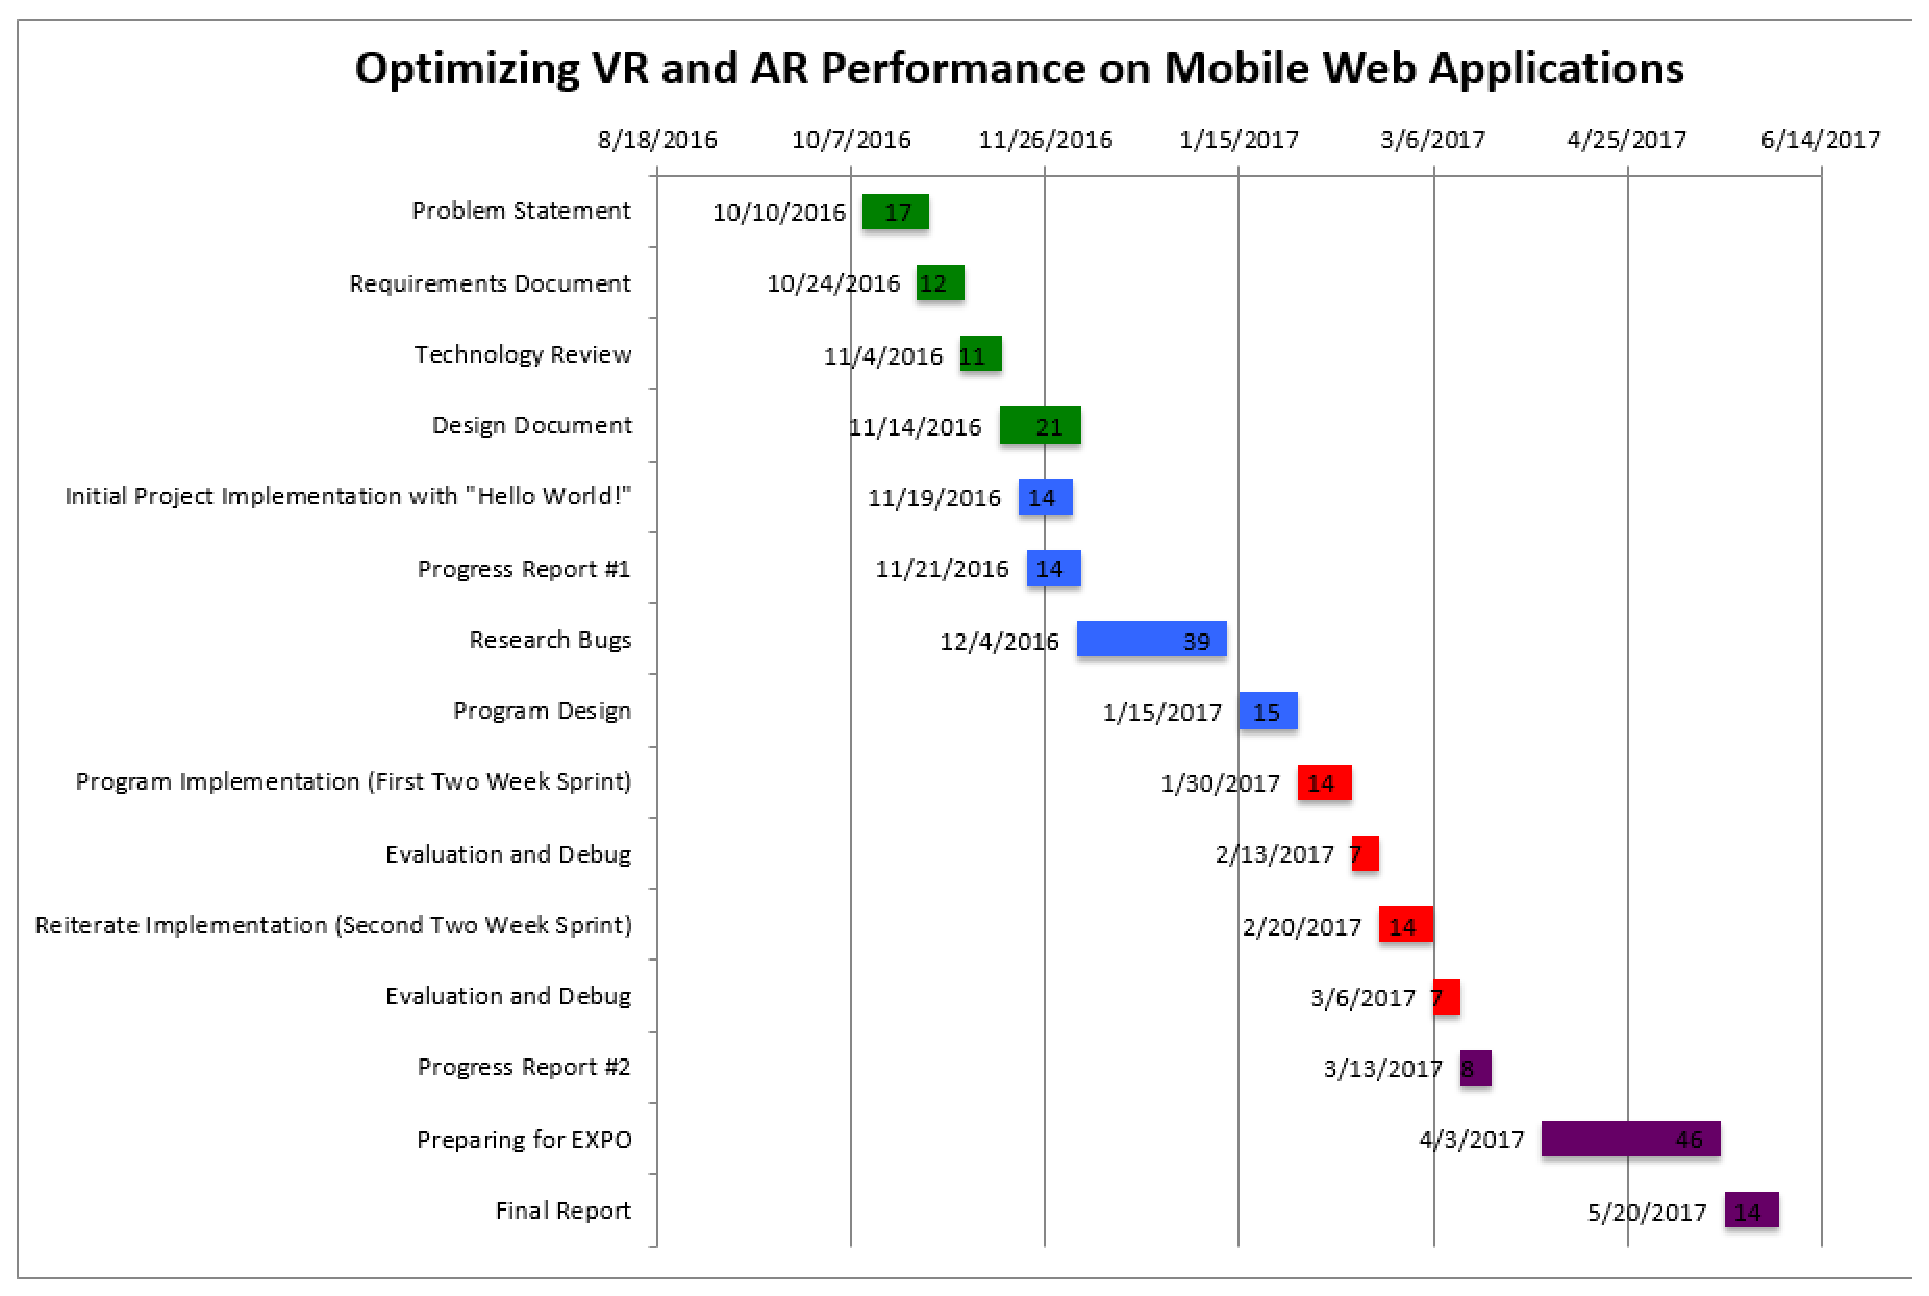
\includegraphics[width=\textwidth]{OVRAR_Gantt_Chart.eps}
        \end{center}
     
    \vfill
        
    
\end{enumerate}

\subsection {Changes since the original Design Document}
    \begin{tabular}{ | p{1.5cm} | p{12cm} | }
        \hline
        \textbf{Number} & \textbf{Changes and Comments} \\ \hline
        \textbf{1} & Found a more user-friendly web hosting platform; replaced Apache with the home directory server space for every OSU engineering student    \\ \hline
        \textbf{2} & Updated the Design Document to reflect changes in programming schedule; added alpha release and updated sprints. \\ \hline
        \textbf{3} & Updated Design Doc to reflect change in development environment; VS -> notepad++ \\ \hline
        
        \hline
    \end{tabular}
    \smallskip

\newpage
\section{Tech Review}
\subsection{Original Tech Review}

\begin{enumerate}
    \item Generation Of Scenes In Browser 
    \begin{enumerate}
        \item Options to Use \newline
        The options for browser scene generation are: Internet Explorer, Google Chrome, Mozilla Firefox, Opera, and Safari. 
        
        \item Evaluation of Options \newline
        Each of the web browsers are capable software applications for retrieving, presenting, and traversing information resources that are not only identified by a URL but an IP address as well and are capable of hosting a web page, image, video, or other piece of content such as 3D imaging.\smallskip
        
        \item Options Comparison \newline
        While each of these options are testable web browsers, they may require different coding aspects and each option might require different libraries or coding tactics (i.e. Explorer does not like certain HTML and CSS variable phrases and structures that chrome and Firefox do) and would require extra time and effort to transition code. That being said, it would allow for more robust research should we be able to verify the bugs we encounter through multiple browsers.\smallskip
        
        \item Discussion \newline
        Though we may be able to test in each of these browsers, our client has asked us to use Mozilla Firefox because it is the browser environment that our research project is based around and that is the company our client works for. However, once we encounter bugs, we will attempt to verify them in multiple browsers to get a better understanding of why that error arose in Firefox and if it is singled out there, or expands across multiple browsers. \smallskip
        
        \item Selection \newline
        Mozilla Firefox \\
   
    \end{enumerate}
    
    \item Processing/Analyzing Data 
    \begin{enumerate}
        \item Options to Use\newline
        Options for the recording and analyzing of data are: Excel, Google Sheets, Apache OpenOffice, LibreOffice, and many more.\smallskip
        
        \item Evaluation of Options \newline
        Each of these tools are used for analyzing and recording data and some over others are better at manipulating data to either find patterns of present trends. Excel and google sheets are simple computer software programs that are used for storing, organizing and manipulating data. Apache OpenOffice is a software suite for word processing, spreadsheets, presentations, graphics, databases and more. \smallskip
        
        \item Options Comparison \newline
        Though each of these options are capable of recording general data, some of them offer more features then others and some are more complicated than this project's data recording needs to be. Apache OpenOffice and Libre office, for the time being, seem beyond the scope of our data recording needs. The type of data we are going to be recording analytics and number comparisons, which Excel and Google Sheets are perfect for. \smallskip
        
        \item Discussion \newline
        So without needing fancy data analytics tools, we simply need a place to store the data we record which will be software and hardware specs. We are going to need to store large quantities and have them readily comparable against different parameters, which the spreadsheet aspect of both Excel and Google Sheets provide. That being said, Excel offers more design, formatting, and general mathmatical capabilities should we require them in the future. \smallskip
        
        \item Selection \newline
        Excel \\
        
    \end{enumerate}
    
    \item Setup Local Host Server
    \begin{enumerate}
        \item Options to Use\newline
        The options for setting up locahost servers are: Nginx, Apache, and Lighttpd.\smallskip
        \item Evaluation of Options \newline
        These are the three most used free web-servers provided by the open source community, making up over 50\% of domains, that will allow of to remotely connect via mobile web-browser through IP address. \smallskip
        \item Options Comparison \newline
        a) Nginx, the second most popular web hosting server software supports most OS and uses event driven architecture instead of threads. \newline
        b) Lighttpd is the third most used server software but serves less than 1\% of domains and is also event-driven. \newline
        c) Apache is the most used server software with it being used on 60\% of domains and it supports a multitude of packages. Additionally it is easier to install and provides for a much richer and reliable environment.\smallskip 
        \item Discussion \newline
        Because we don't know the situations we are going to run into through our web hosting, we are going to want as server host that is not only more reliable and easier to use, but we are potentially going to want to apply different packages, and because apache holds the majority of user use, we can trust that it will be able to cater to our needs and have more up-to-date features. Additionally, the extensive documentation already online regarding Apache will potentially help us in troubleshooting the errors we run into and will allow for much quicker and hassle-free fixes.\smallskip
        
        \item Selection \newline
        Apache \\
    \end{enumerate}
    
    \item Generation and capture of the data\newline
    The biggest part of our project is the generating the data we receive in our test cases, and capturing it so we have good and reliable metrics of performance data to analyze. The challenge that arises from this is when dealing with multiple frameworks of development, such as running this project on the Android OS, on a phone, where it renders multiple test cases through two browsers that are interpreting languages through two different frameworks. If performance issues occur during development, we need to be able to understand where the bottleneck occurs, whether it lives in the OS, the browsers, or the frameworks we're developing on. \smallskip
    \begin{enumerate}
        \item Options to Use\newline
        There's a couple of options to use, specifically we're looking at the Android SDK, which has features that are included with the capturing of data through different levels of the android stack, where there's performance metrics with the phone, the operating system, and within the browser. A competing tool is the Firefox Dev tools, which allows the connection of devices over a network, and will capture performance metrics through the device onto the browser. This holds information such as performance usage, memory consumption and, and rendering speeds of the scene. Chrome Dev tools has similar, competing tools to analyze the metrics when being used to render the scenes on Chrome.\smallskip
        
        \item Evaluation of Options \newline
        Below is a list of functionality that comes with each of the tools (Android SDK \cite{android}, Firefox Dev Tools \cite{firefox}, Chrome Dev Tools \cite{chrome}) to be able to compare and contrast the tools that we will use when generating our test scenes through this project. Each of these tools have more features than what is listed, this is just a short description of what each tool will be useful for us.\smallskip
        \begin{center}
            \begin{tabular}{ | p{4.5cm} | p{4.5cm} | p{4.5cm} | }
            \hline
            \bfseries Android SDK & \bfseries Firefox Dev Tools & \bfseries Chrome Dev Tools  \\ \hline
            \textbf{Performance Monitor:} Allows us to track the memory and CPU usage during rendering, and frames being developed. 
            & \textbf{Remote Debugging:} Firefox allows us to do remote debugging of code that is running in Firefox for Android over a USB connection.
            & \textbf{Remote Debugging:} Similarly to Firefox, allows remote debugging of the code that is running in Chrome for Android over a USB connection.\\
            
            \textbf{Memory Dump:} Allows us to see memory allocations to the device to see where memory leaks occur.
            & \textbf{Performance Tools:} Has multiple tools to analyze processor and memory usage, frame rates, and call trees to see how performance is handled in the browser compared to Android OS.
            & \textbf{Timeline Performance:} Chrome has a tool that will record and analzye all the activity in the browser as it runs, capturing FPS and CPU usage, along with profiling the JavaScript stack. \\
            
            \textbf{GPU Profiling:} An option that allows us to track the time it took to draw the last 128 frames.
            & \textbf{Source Editor:} Allows us to make quick edits to our source code during runtime and see performance or visual changes.
            & \textbf{JavaScript Debugging:} Explicit tools for JavaScript debugging, allowing us to step through the code, sets breakpoints at predetermined intervals, and watch variables during runtime.\\
            \hline
            \end{tabular}
        \end{center}
        \smallskip        
        
        \item Discussion \newline
        These tools will all actually be used simultaneously, as they are recommended by our client to test multiple tools as we conduct our research. The tools all have a set of performance analysis built into them, which allows us to be able to capture the performance metrics while we test in multiple environments. Each tool has special features specific to each browser, which will help during debugging, and pinpointing areas that are causing performance issues that may occur in different areas of rendering (OS level, browser level, or JS/interpreter level). More tools allow us to have a wider set of test cases to determine possible areas of optimization issues and bottlenecks.\\
                
    \end{enumerate}
    
    \item Generation of Scenes on a Mobile Device\newline
    How the scenes will be rendered, and the choice of which device was predetermined for us already. Our client informed us that it would be beneficial to testing if they were all conducted on the same device, the same device used with other teams that are similarly working on the A-Frame framework. This reduces the amount of variables in testing, especially when the devices has different specifications and may handle scenes better or worse than the devices they use. It helps us pinpoint specific areas in testing where bottlenecks occur when attempting to render the scenes on the phone.\smallskip
    
    \begin{enumerate}
        \item Options to Use\newline
        Since our client requires us to use a specific mobile device to have the same device and have similar testing case for our research, the Nexus 5X is one of the newer phones that came out last year, and has substantial hardware specifications to handle the rendering of graphical scenes. As the project is developed on the A-Frame framework, and implemented through the Firefox and Chrome browsers, the Android OS platform is the most supported for this kind of testing and development. Safari and iOS are excluded from this testing due to issues with A-Frame running on Safari, that research is outside of the scope of our project, and because of this, iPhones were obviously excluded as a choice of hardware for development purposes.\smallskip
        
        \item Evaluation of Options \newline
        The only option is the Nexus 5X, as this is what our client requires us to use for testing development. Though for the sake of comparison \cite{phonespec}, this device is best for our testing development because it allows a wider range of test environments due to the powerful hardware specifications and the platform it was built on. In the comparison below, the hardware specifications the newest generation iPhone 7 and the LG Volt device will be compared.

        \begin{center}
            \begin{tabular}{ | p{4.5cm} | p{4.5cm} | p{4.5cm} | }
            \hline
            \bfseries Nexus 5X & \bfseries iPhone 7 & \bfseries LG Volt  \\ \hline
            \textbf{OS:} Android 7.0 "Nougat"
            & \textbf{OS:} iOS 10.1.1
            & \textbf{OS:} Android 5.0 "KitKat\\
            
            \textbf{Battery:} 2,700 mAh Lithium Battery
            & \textbf{Battery:} 1,960 mAh Li-Po Battery
            & \textbf{Battery:} 3,000 mAh Li-Ion Battery \\
            
            \textbf{RAM:} 2 GB DDR3 Memory
            & \textbf{RAM:} 2GB DDR4 Memory 
            & \textbf{RAM:} 1 GB DDR3 Memory\\
            
            \textbf{CPU:} 1.8 GHz Hexa-core 64-bit Processor
            & \textbf{CPU:} 2.34 GHz Quad-core 64-bit Processor
            & \textbf{CPU:} 1.2 GHz Quad-core 64-bit Processor\\
            
            \textbf{GPU:} Adreno 418 @ 600 MHz 
            & \textbf{GPU:} Apple G9 
            & \textbf{GPU:} Adreno 305 @ 450 MHz\\
            
            \hline
            \end{tabular}
        \end{center}
        \smallskip
   
        \item Discussion \newline
        As shown in the table, the Nexus 5X is a very capable phone to handle the rendering of graphical scenes through the browsers. Compared to the other choices shown, it is stronger or similarly comparable in hardware specifications to the newer iPhone, and the LG Volt. Along with uniform testing platforms, the hardware on the Nexus 5X will be reliable enough to generate substantial test cases that can be used on future iterations of mobile devices as the hardware becomes stronger and more efficient. It's logical to test on best hardware for the time, as the hardware will become deprecated within a couple of years.\\
        
    \end{enumerate}
    
    \item Version Control and Documentation\newline
    Our deliverable product for this project will be a report detailing the results we've found through our sets of test cases, and so having proper version control and documentation is a key thing to have for this project. We have a need to be able to have information readily accessible to us for when we are dealing with multiple test cases, to be able to review previous results and data to be able to determine the cause of possible bottlenecks that occur in real time. We need to be able to reference our findings, import and export the data in a fashion that would not mess with the formatting of our documentation and handle imported into our choice of version control without issues.\smallskip
    \begin{enumerate}
        \item Options to Use\newline
        In terms of version control, we are going with Github, as it is a requirement for the class. Everything that is developed, recorded, written, and analyzed will be uploaded to Github. This will encapsulate the entirety of our project. Our documentation can be accomplished a couple of ways, either through LaTeX, Microsoft Word, or Google Docs. Since our documentation is being uploaded to Github, it's essential that our choice of tool meets the requirements of being easily accesible, not ruin formatting, and imported/exported easily into our version control. Each of these tools have their own purpose, and will be detailed below.\smallskip
        
        \item Evaluation of Options \newline
        Microsoft Word is probably the most widely used version of word processing, but has issues when importing and exporting to Github. Since Github essentially parses line per line and uploads the differentials of added/deleted lines every time the document is committed, this makes it difficult to understand what lines were changed in the document. Also when attempting to importing data tables and graphics into Word, it will make formatting as an unnecessary chore.
        \newline
        Google Docs is a free version of version control of documentation and word processing all in one, but comes with a caveat of only really working within itself. Attempting to export the files processed in Google Docs will mess up with formatting, and will not be easily parsed into our version control, where needing to see up to date documentation will become even more unnecessary work. While it does attempt to create a form of version control, it only adds to being an extra place to "check" for up to date information, and the word processing formatting for it just does not fit within our scope for this project.
        \newline
        LaTeX is a mark-up language, similar to HTML. As a word processor, it breaks down the formatting based on the packages included into the file, and the defined parameters allow uniform formatting in all specifically defined areas. Even graphics will be easily imported into the document, as tools such as PSTricks allow the rendering of the images based on a few function calls in the document, and when compiled it will generate the file properly. This fits in the scope for our project as it will fit within the use of our Github version control, and will allow us to see the changes made to the document and view them in real time. It's also very trivial to add special tables of data or analytical images as it is just a file with marked up text where formatting is already predefined.\smallskip
              
        \item Discussion \newline
        Documentation is done very trivially and the compiler for LaTeX handles formatting for everything else. The results are very predictable and the ability to view the contents of the actual .tex file and the resulting .pdf file allows for easy portability and readability into the version control we are using. LaTeX makes it also very trivial to import tables and images into it, when it comes time to generate the analyzed data that we receive for this project. Every other option we discussed has some unnecessary challenges when implementing our results into our documentation. They have too many downsides, while LaTeX fits into the version control scheme very easily.\\
        
    \end{enumerate}
    
    \item Creation of Scenes in A-frame
    \begin{enumerate}
        \item Options to Use\newline
        As the purpose of this project is to determine areas of development within A-Frame where practices will be best used, so we are going to use A-Frame to create scenes. A-Frame is an open-source WebVR framework for creating virtual reality (VR) experiences with HTML with the use of the Three.js framework.\smallskip
        
        \item Evaluation of Options \newline
        A-Frame will handle the specific Three.js calls to help render the scene with 3D objects with the use of WebGL API. The WebGL API utilized by Three.js will interact with the hardware processing when drawing the topology of polygons, textures, lightings, animations, and scenes to the viewport. There are three things about A-Frame that are important to our project:
        \newline
        a) A-Frame is a framework for reworking Three.js implementations to make the calls to draw 3D scenes simplified by using HTML.
        \newline
        b) A-Frame Takes the marking A-Frame tags and produces the proper JavaScript calls to generate scenes to the browser.
        \newline
        c) These calls are the input information to the Three.js framework, which outputs the polygons and scenesto be drawn.\smallskip
        
        \item Options Comparison \newline
        A-Frame is the only option we have, since it is the requirement of the project, and not other frameworks fit in our scope of the project. 
        \newline
        A-Frame is an open-source WebVR framework for creating virtual reality (VR) experiences with HTML. We are able to build VR scenes that work across smartphones, desktop, the Oculus Rift, and the room-scale HTC Vive.\smallskip
                
        \item Selection \newline
        Based on all the points mentioned above, we are going to use A-Frame to create scenes. \\
    \end{enumerate}
    
    \item Development Tools
    \begin{enumerate}
        \item Options to Use\newline
        In order to develop a software project as a group, one biggest point is to choose the right development tool. There are a few good development tools for software, such as Visual Studio, Notepad++, Sublime, and so on. We will evaluate and compare with one from another, and decide which is the best choice for this project.\smallskip
        \item Evaluation of Options \newline
        Visual Studio offers a comprehensive development environment to help Web developers build standards-based Web applications and services. It improves productivity by allowing users to rapidly develop, test and deploy Web solutions. Additionally, Visual Studio offers a free version aimed at Web developers. With Visual Web Developer Express, you get a full featured web development environment for working with ASP.NET, Javascript and Web standards.
        \newline
        One of the main advantages of Notepad++ is that it requires no training and you can start HTML straight away. It comes free with every version of Windows which means you do not have to go through the hassle of downloading the program. The program doesn�t take up much space on the laptop/desktop PC and because it�s low specification software it means that it doesn�t take a long time to load.
        \newline 
        Sublime has got a modern and colorful interface. It also has full screen support, and uses the �Minimap� feature pretty well which makes you deal efficiently with files carrying thousands of code lines. Plus, distraction free Mode that makes you more focused on Another advantage of sublime is it can auto saving of your code to keep you worry less and the Spell Checker doesn�t let you make errors while writing codes. Besides, availability of Multiple Selections will eventually simplify your task.
        One big disadvantage of sublime is that its license costs \$70, which makes it an expensive deal than many other code editors. \smallskip
        
        \item Options Comparison \newline
        The goal of Visual Studio is to provide rich development tools to all developers globally on any platform. Development teams will be able to develop software for Web, mobile, server and desktop with Visual Studio. Also, it also has an online version ,Visual Studio Online, which is a set of tools that makes it much easier for continuous integration across different platforms.
        \newline
        Of the free options here, Notepad++ is extremely popular. It is often mentioned in blog posts as a great free option for someone just getting into code editing or who needs to edit a few files here and there (but who probably don�t want to buy an expensive or complex editor). Notepadd++ is a wonderful, simple option not just for beginners but developers at any level.
        \newline
        Sublime text is a beautiful, feature rich option for code writing and editing. A big draw for this editor is the fact that it puts a premium on user experience. This includes features like distraction free writing mode, quick shortcuts/search, split editing, and so on.\smallskip
      
        \item Selection \newline
        In this project, we are going to use Visual Studio as the development tool as Visual Studio is often used to develop computer programs for Microsoft Windows, as well as web sites, web applications and web services which our project is mainly focus on.\\
        
    \end{enumerate}
    
    \item Language Tools
    \begin{enumerate}
        \item Options to Use\newline
        An implementation language is a formal computer language or constructed language designed to communicate instructions to a machine, particularly a computer. Understanding difference(s) between programming languages is crucial. If wrong language is chosen for a project, it will take a lot of time and efforts to change the course and re-implement the project or its part in different language. For our project, since we are going to test the performance of web app through A-frame, which is a Web framework, so we should choose from the languages that are specific to web development. A few examples are HTML, Java Scripts, and PHP.\smallskip
        
        \item Evaluation of Options \newline
        HTML is easy enough to write, but errors can be costly. Another disadvantage is the time it takes to choose the color scheme of a page and to create lists, tables and forms. An advantage to HTML is that it is easy to code. Much of the code can be customized by someone who knows proper HTML formatting. HTML also allows the use of templates, which makes designing a web page easily.
        \newline
        JavaScript is very fast because any code functions can be run immediately instead of having to contact the server and wait for an answer. Plus, JavaScript is relatively simple to learn and implement, and it plays nicely with other languages and can be used in a huge variety of applications. Additionally, being client-side reduces the demand on the website server. However, since JavaScript code executes on the users' computer, in some cases it can be exploited for malicious purposes. This is one reason some people choose to disable JavaScript. JavaScript is sometimes interpreted differently by different browsers. Whereas server-side scripts will always produce the same output, client-side scripts can be a little unpredictable. 
        \newline
        One advantage of PHP is that it has both procedure programming language and OOP language features. This mainly attributes to its evolution along the way. This means that programmers from different programming language background can pick up this language within short period of time. Its disadvantage also comes from its ample language features. Some libraries written by a programmer from a procedure programming language may be difficult for programmers with an OOP background to maintain.\smallskip
        
        \item Options Comparison \newline
        HTML, stands for Hyper Text Markup Language, is the standard markup language for creating Web pages. It describes the structure of Web pages using markup, and its elements are the building blocks of HTML pages which are represented by tags. HTML tags label pieces of content such as "heading", "paragraph", "table", and so on. Browsers do not display the HTML tags, but use them to render the content of the page
        \newline
        Programs written in JavaScript run in the web browser itself, so if the website has a JavaScript program, the program will be automatically fetched by your visitor's browser and executed on his/her computer. 
        \newline
        PHP programs, on the other hand, run on the computer where your website is located, that is, on your web host's computer. After the PHP program does what it needs to do, it sends the result to the visitor's web browser, which merely displays the results. \smallskip
        
        \item Discussion \newline
        As this project serves as to be used as research, correctness will be based off of how well we can push the boundaries of our software, based on the performance the hardware can provide. Therefore, we need to collect the information in different types of implementations between scenes the program generates, so we should be able to understand and write some test scripts. \smallskip
        
        \item Selection \newline
        We are going to use HTML, JavaScript, and PHP simultaneously, as all three of them are very crucial to understand our project. We need to understand these languages in order to find the bottlenecks, where the optimization needs to be done. \\
        
    \end{enumerate}
    
    
\end{enumerate}

\subsection {Changes since the original Tech Review}
    \begin{tabular}{ | p{1.5cm} | p{12cm} | }
        \hline
        \textbf{Number} & \textbf{Changes and Comments} \\ \hline
        \textbf{1} & Updated to reflect server change    \\ \hline
        \textbf{2} & Decided to change our Development Tool from VS to Notepad++; easy to utilize in our situation \\ \hline
        
        \hline
    \end{tabular}
    \smallskip

\newpage
\section{Team Weekly Blog Post}
Over the past three terms, each of us has submitted weekly updates to describe the progress over the past week, the problems we encountered during the week, and the plans we have for the next week. This is to keep track of our progress as we move through the project time-line, and determine whether we are on track, or behind our current schedule.


\subsection{Charles Siebert}
The following sections include weekly summaries and a retrospective reflection over the past three terms for Charles Siebert.

\subsubsection{Weekly Summaries}
\begin{itemize}
    \item Fall Term:
\newline
Our group picks up this project at the start of week three of this term, since the projects were assigned the week before. We met for the first time this week to have our first meeting with our client to discuss the overall scope of the project. During this week, we had to make a Problem Statement that presented the project as a solution, or adding to a solution to a problem. This project specifically is about researching and optimizing an open-source framework that renders virtual and augmented reality scenes onto mobile devices. During this week, we didn't run into any problems in writing the Problem Statement, and our client was pretty clear in the purpose and scope of the project. Our challenges for the next week is understanding what needs to go into a Requirements Document and start thinking about how to approach implementing A-Frame onto mobile devices. Our client discusses with us about testing development on standardized equipment that they use, to reduce discrepancies, so he is sending us Nexus 5X phones.
\newline\newline
The next coming week, in week four, we plan on setting up the phones we received to be used as tools for this development process. We talked after out meeting with our TA about learning the tools to use and get set up with the Hello World project in A-Frame. Since the last week, we've received feedback on our Problem Statements to revise it once more, and received the requirements for producing a Requirements Document for this project, that will be uploaded to this project's repository by October 28th. When Roger and I contacted our client in the weekly meeting, we discussed the goals of the coming week and will reconvene next Monday about our progress. We haven't had any problems this week, as being in contact with our client and group members hasn't been an issue.
\newline\newline
Starting at week five, we are going to be finishing up our revisions to the final version of our Requirements Document. After we revised the Problem Statement and re-submitted with the proper signatures, we received an extension towards this next writing assignment. We didn't meet up with our TA at the end of the week, due to other circumstances, though we did meet with our client to talk about the upcoming work we are producing and what the document entails. During the week, we started putting together our Requirements Document, which seemed to pose a problem due to missing a session of class to properly evaluate the kind of content that goes into it. Missing a time for our group to meet made it hard for us to communicate and properly plot out a Gantt chart to describe how the coming months will play out. Our next meeting with our client is on Tuesday to go over the progress we've made and talk about how the coming week looks like.
\newline\newline
In week six, we had to work hard on our Requirements Document, as it is due very soon, with our clients signature. We received back our problem statement, which had a low scoring on it, so we went to discuss it with Kirsten during her office hours. We were able to find out that the wording was stated as a real life problem, when we're on a research project rather than producing an item for consumers. We plan on starting to work on figuring out how our initial implementation is going to work, as we have to decide on the system to host a local web server, and connecting remote debugging on our mobile device. There haven't been any problems this week, as we have planned out the work needed to get our requirements document finished.
\newline\newline
During week seven, I worked on the revisions of the Requirements Document with our client, discussing some issues that were unclear, or heeding his advice on the length of certain sprints that we have planned out in our time-line for our project. Though we tried to have revisions and a final version turned in on Friday the previous week, it's good that we were able to discuss some pertinent details and concerns that our client had. Aside from this, we worked on discussing the parts of the Technology Review that we have to put together, all in which we have 3 parts that we are responsible for. Our plan for the next week is finishing the Technology Review, which is due on Monday, and start the planning process for our Design Document. We have a meeting with our client on Monday to discuss in detail some of the technologies we need to utilize based on the constraints of our specific project. Overall, the biggest challenge we faced was finishing the revisions for the Requirements Document while simultaneously attempting to piece together the things we need to write for the tech review. The added time to send the document back for clarification and confirmation on the unclear sections will add some time to the process.
\newline\newline
In week eight, we were unable to properly finish the Technology Review in time on Monday. We received an extension on the assignment so we can finish the assignment and turned it in on Wednesday at noon through the GitHub repository. One of the classes this week was cancelled, which gave us some time to look through the sections of the Design Document, and determine which parts of the system we need to describe in detail. During the cancelled class time, we were able to commit a bare bones document to start off with the Design Document to our GitHub repository. We talked with our client and discussed some technologies that their other teams have used to track the performance metrics through web-browsers on phones, which led us to some good information to include and discuss in the documents. This coming week, we have to prepare for the last few assignments for this term, of which include the Design Document, Progress Report (Term 1) and the poster, which are all pretty time consuming. Currently our focus is getting the first revision of the Design Document out as soon as possible to get feedback as early as we can to avoid the situation we ran into with the Requirements Document (time delays between revisions caused some issues). Though this is Turkey Week next week, I will have some time to work on this during the times I get tired of my family. We didn't run into any pressing issues this week, but I do think we will have some trouble finding time during dead week and finals week to finish all of the stuff to end this term. It's essential we get some of the pressing matters finished as soon as possible.
\newline\newline
Since week nine has a holiday, we had little time to meet up and coordinate. It was discussed that we would make headway on the documents we need to prepare and work on our progress report that's due at the end of the term. The past week I worked on a bit of my part of the presentation and discussed how we will piece together the progress report and video, and it looks like we'll be using OBS (Open Broadcast Software) as our tool, since I've had previous experience with it. The next week, we need to have a finished version of our Design Document by Sunday at the latest, for our client to go over in time for it to be turned in on Friday (Dec. 2nd). Our challenges we face is getting enough time to meet together and get these documents all pieced together, since we have two papers, a 30 minute presentation, and a poster we need to fulfill within the span of eight days.
\newline\newline
In the last week of the term, we had to work to get the Design Document done in time, and have it polished enough to send off to our client. We finished the Design Document, and turned it in without our client's signature as we are still waiting for a response for some feedback or revisions. The design document itself lists out the concerns of the project, where we need to determine how to overcome these concerns based on our design decisions we make. This included the tools we are using, methodology of implementing and re-implementing, and ideas of how we are going to stress the resources we have in order to determine areas of optimization and bottlenecks. Since it is the end of the term, this is a harder deadline. We planned out what to do for the rest of the term, in terms of the poster and progress report. Essentially we are meeting up during the weekend to record our presentation for our project, where we will make and use our sections of PowerPoint slides to talk about. The challenges we face for the coming week is to find enough time to be able to write all the slides, record enough interesting content, and then still be able to put together a mock-poster and the final progress report. Though we do have a challenge over the winter break, and that's to not get distracted from the project and stay on course. We plan on doing research on the bugs currently found within A-Frame and Firefox specifically, and start our initial, simple implementations of A-Frame onto our mobile devices. This will help us in understanding the work flow that is required for this project over the coming months.


\item Winter Term:
\newline
Being our first week back, we were just catching up with each other on the progress that we made over the break. I had gotten an HTC Vive over the break (the Vive is outside of this project's scope), but I was able to manage on getting A-Frame content to be displayed through the HMD on the VR kit. This had to be accomplished with using the experimental builds of Firefox (Nightly) and Chrome (Chromium), which is the technology we are using to test and render our scenes. With this motivation, I was able to set up A-Frame content on my own web server hosted by Oregon State, and tested to see if it works on our own host, and tested if it would display then. It did, with very little issues. I was able to tweak the "Hello World" version of their framework by adding simple transformations, animations, and additional objects to become accustomed to how the framework interacts with the HTML tags and Javascript declarations. The work that we have to produce over the coming two weeks is to properly design our testing implementation for the framework in the scope of mobile phones and devices. We have two weeks planned for the designing phase to properly make sure we include as much as we can within the time we're given. For the scope of WebGL being rendered on phones, we have to determine what possible vulnerabilities the devices may have in rendering the scenes compared to their laptop/desktop counterparts. We have an idea on how we'll split up the work, and how the testing will go, but the details of what inefficiencies we need to test need to be fleshed out at this point.
\newline\newline
During the second week, our group met up on Saturday to start fleshing out the details of the design of our project. We determined that the structure of the project will be testing different implementations of scenes in separate "rooms" (the rooms are essentially new web pages to be loaded and rendered), so we will have the user walk through the scene to reach these new rooms to load up a new testing scene. Right now we have considered four possible scenarios to test, and we're thinking of an inclusion of a "hub" room that connects to each test, where it will have basic descriptions of the project scope, what each room does and tests, and citing further information on the project. The tests we are considering include: "high polygon" objects (rendering large amounts of vertices, face normals, and lighting), large amounts of texturing on objects, animation calculations through simulated physics, and a mix of everything mentioned. Our approach to this design is to find the limits of the mobile device with common graphics programming based on each individual implementation, and the final test would be including all of the tests in a manner that would be within a realistic scope of another programmer's work. We understand that someone isn't going to make and publish a program that just has objects scattered everywhere, but we think it would be beneficial to understand where we can, or can't, break the devices in order to shape our testing environment that would work for everyone else. This also allows us to cross-reference performance discrepancies between implementations to determine if performance is hindered in one area and not in the other We met with our TA on Wednesday to discuss our progress, and where we stand within our project, and it sounds like we are on good grounds to finish by the end of Winter term, and we will have to keep in mind our roadmap that we have planned out last term to make sure we don't fall behind. Our challenges we face is keeping ourselves to our pre-made deadlines to make sure we produce quality work in the time we've allotted for ourselves. The things we need to work on over the next week is to finish polishing our design for our project, to make sure we're all on the same page on what needs to be done, and how it will be done. It's important to have this fleshed out so we aren't wasting our development time attempting to debug our implementations, and have enough time for proper testing.
\newline\newline
As we enter the third week, we went over a couple of meetings, and talking with our client about our design for the project. He gave us some feedback on areas that we described some issues, such as setting up a localhost server properly, and feedback on our testing methodology. He said having separate rooms testing a single thing was good, and then to combine them would work. We plan on starting our development this very next week, but currently we are working on getting everyone on the same page with the topic of actually developing this. We are working on covering the basics so we can discuss these things and move forward more clearly. Our challenges for these next two weeks (our first development sprint) is to accomplish two room to start our testing rounds. Our problems that we face is that working with this new framework, we will encounter some development issues (learning or debugging) that might slow down our progress. Though working through HTML and JavaScript, learning should hopefully not be a big issue.
\newline\newline
Going into the fourth week, we have been working on our initial implementation of our project. Currently in our two week sprint we plan to have two of the four rooms in working condition in time for our alpha release. At that point, it should serve the purpose of the analysis that we will be giving from the data we are collecting for this project. I personally have been working on setting up the initial rooms. I have some progress into this, but ran into a couple of issues with the Scene Inspector feature in A-Frame, where it wouldn't export the added properties to the entity. I have some information compiled on this and could be a bug, and will look into if it's already reported or not. During the week, we discussed the future deadlines of the course, and determining what assignments will need to be done for the end of the term. At the end of this sprint and initial data collection and analysis, we should have an alpha release and enough information to create a conclusion. The problems we face for the next week is to finish our first implementation to stay on track. The two rooms we're working on are are simple enough to make our testing platform hit maximum resources used. We need to iron out who will be taking care of handling all of the expo information, and planning out our midterm video and progress report, as they will generally take some time to compile and render all of the information.
\newline\newline
In week 5, we are working on getting everything in the alpha release. In our design plan that we discussed earlier in the term, we wanted to separate the types of features to determine how they specifically have an impact on the system. For example, we want to see how overloading the phone and scene with hundreds of objects, and how we can determine exactly is causing the performance issues. The four rooms each have a purpose to collecting specific information based on that implementation. Room 1 specifically handles object loading and displaying high number of vertices and polygons to determine if the constant redrawing will have any affect on the performance. Room 2 handles animations, which deal with the constant recalculation of points and normal vectors off of the polygon's faces, where if we see possible object interactions, we might see further performance decreases in the CPU, rather than the previously discussed GPU. Room 3 handles user interaction and varying density and lighting intensities, basically handling the lighting calculations aspect as this will allow us to turn on or off lights to see how linearly adding lights could push the performance boundaries, as lighting is very computationally expensive. The last room is just getting everything put together, and how the scene will render with everything interacting with each other. This will be interesting because it serves as a way to cross-test these implementations and could determine if performance exponentially gets worse or even better. My plan at this point is to finish getting the ability to load our own objects into the scene and randomly generate them across the scene. We're deciding to create a sort of a forest scene that would be familiar for most people to see. So in this Room 1, we're just creating a forest of trees and better ground texturing. I ran into some issues when attempting to add a component feature that was listed in a new release of the A-Frame framework, but failed to recognize I was still developing on an outdated version, and inevitably ran into getting frustrated over a simple oversight. Oh well. We are also working on delegation of work, which is working out well when having development separated into these different rooms. We can work alongside each other on the framework itself, but don't run into each others heads when making these rooms. As long as we stay in the scope of the rooms and their purpose, we're pretty much free to sculpt the scene as we want it, and it makes for some interesting results when putting them all together! Over the next week, we need to determine how to delegate all of the writing, and video editing, and still have time to record all of this new information we need to provide, as we are finishing the development for our alpha build.
\newline\newline
In this last week 6, we were running around getting the polishing touches ready for our alpha release. This alpha release is consisting of four total rooms that we consider to be substantial areas of computer graphics to stress test on the phones that were provided. The challenges we ran into getting this ready is constant updates that keep occurring with A-Frame in such a short time period, which is a good thing! But some features that we needed (link traversal) was implemented in an early build of the framework, in which there was documentation for that build specifically, but was taken away to be better improved. We put together all of the features into the final room, and set up the scene. All of the other rooms are finished and ready to start the analysis and testing as the project moves into the alpha release state. We properly managed to delegate the work in recording all of our speaking parts for the progress presentation, and still managed to be able to video edit, write all of the new slides, create the progress report, and help compile the OneNote stuff in time. Over the next week, we have a challenge in how we're going to collect and organize all of this information, because I have a feeling it's going to be a lot of information that we will have to analyze. We might have to look into proper planning and workflow in order to obtain the proper information in a timely manner, and exactly how we're going to manipulate it.




\item Spring Term:
\newline
For the first week back, we talked with our client about our current progress, and where we're at with development and how we will proceed with testing. Gave us good feedback based on how we've been moving forward with development, and sounded pretty optimisitic. Over the next week, we will be working with our client to approve the poster we have worked on. There is a second draft of it due soon, and we will need to discuss with our client over any potential brandings they may need to have presented as well. The problems we may run into is getting our test data lined up and ready to determine what we need to find to write and publish our results.
\newline\newline
In the second week, we worked on ironing out some finals bugs before testing. I worked on finding a proper model to compare against our original, and finding out how many trees I would need to put into the scene when comparing the vertices of each model that needs to be drawn. We are close to finishing the final development so we can test and compare all of our scenes together. Over the next week we plan to get together and discuss the test cases we have, and how we will draw conclusions for the results we see. We need to talk to our client about our draft of our poster, as it will have industry represented logos on the poster, and determine if it is appropriate to display at the convention. However, we are finishing up our last weeks in this project.
\newline\newline
Starting in the third week, we are talking with our client about getting our poster approved, and determining whether or not Mozilla needs any specific branding associated with our poster. As we work on final revisions of this, we are planning out doing some extra credit down the line to do with another group, to practice presenting our projects. We're finishing up the last of our rooms to push towards testing.
\newline\newline
During the fourth week, we were given the assignment to do a WIRED style article with another group member. Having to interview another classmate in a different group and write about it will help prepare for a different style of writing. As I'm not used to an article style of writing, it is good practice for when we have to write our blog post for Mozilla, as that is one of our main deliverable products for our client. Though having to do it during the code freeze makes it difficult to prioritize everything properly. Over the next week, we have to finish our code before the code freeze hits, and make sure everything is submitted. That means we have to have our poster ready, approved, and submitted. The troubles we may find over the next week is getting everything submitted and finished on time, as we also have to plan our interviews with other classmates.
\newline\newline
During the fifth week, we worked on finishing the code on our project for Monday, as that was the code freeze. The previous week, we were given group member's to do the WIRED article, which required us to interview other people and talk about our projects. Earlier in the week, we also met with our client to discuss the project, and our poster. He also discussed the plans of doing a Mozilla blog post to wrap up the project, which will discuss an abstracted overview of our entire project and our results. We are currently working on fine turning our results data in the next week, and prepare this information for expo and our article for our client. The problems we will face into is getting all of the writing done, as we will have another set of progress reports that we will have to write out, on top of preparing for expo and delivering the rest of our requirements to our client.
\newline\newline
In week six, I worked on getting a Blog article written up to our client to submit for our project. It depicted our approach and resolution based on our testing that we did. Currently working on setting up an account for the Hacks Blog website and submit it for revisions before we can post it. For the next week, we have to get our midterm progress report completely up to date. Have to gather up recording and render a quick video to go with the writing. After that, we have to confirm that we are getting all of the materials we need to prepare for EXPO, which is coming this Friday. Maybe a little practice on our pitches might benefit us... The troubles I see facing the next week is getting this midterm progress report finished, as we have to record and render a new video, on top of submitting a document. Also EXPO is leaving me a little nervous, as it's finally happening.

\end{itemize}

\subsection{Branden Berlin}
The following sections include weekly summaries and a retrospective reflection over the past three terms for Branden Berlin.
	
\subsubsection{Weekly Summaries}

\begin{itemize}
    \item Fall Term:
\newline
It was during week 3 that we were told we had been assigned to the Optimizing Virtual Reality and Augmented Reality Performance on Mobile Web Applications. From then, we made contact with our client Dietrich Ayala and and scheduled weekly meetings via Skype.
\newline\newline
During week 4 was when we actually had our first meeting. We had recently submitted our Problem Statement for the class but were still not entirely sure as to what our project was going to involve, so we made that the topic for our first Skype meeting. During the meeting, our client gave us not only the un down of our project, but the background for it, why we were doing what we were doing; basically the current forms of VR are expensive and unobtainable, however, most people have mobile phones. So Mozilla is setting out to make VR and AR a feasible for mobile users through web applications. We were then told our project would be research into the current capabilities of it and to basically find current issues with it.
\newline\newline
The following week we received our Nexus phones that we will be testing on and planned to get it set up. Our client gave us a basic run down of what we were going to be using on the phone, which were basically debugging tools and various Firefox web browsers. Additionally, we revised our problem statement based on the TA's response to what we originally had, however, we were not able to meet with him this week and were not able to have one last approval, but we mostly had it finished and began the bare bones for our requirement document for the following week.
\newline\newline
For week 6 we received our Project Statement back one last time which required a few more revisions on its verbage as well as its purpose as a whole (research instead of product). We planned to make the changes the following week and turned in for review, but instead we were not able to get it in until week 9. Additionally, for the next week we will be setting up our environments and hopefully get the basics down of our project. By the end of this, we hope to be able to link our phone to a computer server's web page via our local IP.
\newline\newline
During this next week we worked more on revisions for our Requirements Document along with our client to get it to a way he approved of, which took quite a few revisions. This showed us that we didn't actually fully understand our project like we thought we did, but through our client's recommendations we were finally able to get a solid idea of what it is we were actually going to be researching. We next planned to finish up our tech review. This proved difficult while we were also still working our requirements document but we were able to finish it up in the end and learned a valuable lesson in time management. 
\newline\newline
During week 8 we submitted our Tech Document though some requirements came to light last minute, so the final turned in draft was a bit rushed and possibly contained some grammatical errors(on my end). That being said, the final draft was able to cover what it needed to cover and additionally left room for some changes me might run into further down the road of our project when we actually get to the implementation portion. We talked with our client and 1) talked about some applications that we are free to either use or find alternatives for and 2) talked about the applications we would need to use and cannot find change. Our plan for next week was to finish our draft for our design document and start working on our poster as well. 
\newline\newline
For the last recorded week we came back to our original problem statement and made it even more ckea for Kiesten. Additionally, we completed our portions for the Technical Document and got that signed by our client. Our plan was next to next finish up our progress report by Sunday. We divided up the slides based on our knowledge areas for our three subjects and convened to make our recording on Sunday, which went smoothly.
\newline\newline
For Winter break we plan to at least get the Hello World function up and running on our phone. By doing this we will have a huge head start in actually starting our project and it will cut out installation times during actual winter term so we can wholeheartedly focu on actual research and development.


\item Winter Term:
\newline
This first week of winter term was spent going over what we had done over winter break. Collectively, we each were able to get a version of A-Frame's "hello world" function up and running. I personally was able to get it up running, however, I was not able to get my phone to view the web page via an IP address. Since I was hosting the server locally on my computer, the domain was my IP. But after several hours or Port Forwarding, IP declarations, and other non-fruitful endeavors, I realized that using Apache was going to be more of a hassle than it was worth (though it was free). For the coming week, we want to be able to make sure we are all on the same page with the ability to get a web page up and running so we can each start various tests individually. We also want to meet with our client in hopes of finding a good place to start.
\newline\newline
This second week we were not able to meet with our client but we were able to utilize our meeting time anyway. Charles mentioned to me that a good alternative to Apache is simply our school's personalized home directory. This is a school run server that we can post our HTML pages to so we don't have to worry about setting up local servers or anything like that. This has increased our efficiency time immensely and we don't have to worry about that IP issue I ran into over break. Additionally, we agreed on a starting test where we are going to be creating "rooms" that will each pertain to an aspect of a-frame and 3D graphics such that our design will resemble a museum of A-Frame/Mozilla bugs. For the next week, we hope to actually meet with our client to discuss our plan moving forward and to hopefully get some input on our changes as well as his idea on where to go from here. We want to get the green light as soon as possible so we can spend the rest of this term actually delving in to issues.
\newline\newline
In week 3, our client gave us feedback on our initial concept implementation. We had initially presented him with the museum idea where, in a single page, there would be multiple sections utilizing A-Frame and graphic creations. We could then go to each room to showcase and run tests on various implementations and attempt to run different tests in each room. Our client, however, brought up a good point that because the rooms are all in one area, they have a very high potential on conflicting with each other. The amount of memory required in one room would be added to the different room and would not allow us to accurately interpret the information taken from each test. He then offered up different solutions, such as each room being a link to a new page, allowing us to utilize all of our resources for a single test. We hope to get the first stage of development down next week.
\newline\newline
Week 4 Charles went over teaching us how to work with graphics development and showed us a few projects that utilized graphics dev that he had worked on before. This gave us an initial understanding of what we should expect when doing this kind of development and it also give us an initial starting point when thinking about how to test. I have also looked into current A-Frame projects such as Kevin Ngo's github project called "Magicavoxel project". Though this is not in line with an application we will be using, we will be able to at least look at this project to better understand the structure of building a world and working with multiple files in A-Frame. Our next steps are to continue room development and figure out who are lead will be when it comes to taking the responsibilities of our capstone class requirements.
\newline\newline
Week 5 is when we started to get some solid programming done. Charles was able to get up the initial room on our index HTML which hosted two initial rooms containing basic A-Frame features. I then began development on a third room to showcase basic JavaScript features combined with A-Frame. I also utilized D3�s algorithms to throw around object to be manipulated. This week we were able to get a solid foundation for our alpha showcase, but for the next week we planned to add embellishments.  
\newline\newline
Week 6 was dedicated to playing with our foundations to see everything we could do with what we had learned from the previous week. We decided that my room (the initial JavaScript room) was going to utilize object density and object lighting in addition to pushing the limits of JavaScript animations. By doing this, we can push these tools to their max and accurately pin-point what it is about these features that might cause our hardware to falter. This is our last week of development before our alpha release so tried to make the features prettier. Next week is dedicated to revisions and the progress report.


\item Spring Term:
\newline
The first week was spent meeting with our client to catch up from Spring break with any edits or changes we have made, as well as discussing our idea for gathering data. We went over our current design of testing certain features in each room, and how we are going to be doing that. We mentioned we are going to be utilizing Mozilla Beta's dev tools to record the data in our virtual scenes and have them output to a JSON file. Additionally, we will then convert the data to excel and create comparisons. This idea went over well so far, but I think we will truly understand what we are doing only when we begin, because we aren't entirely positive what it is we will encounter until we start our testing. So this next week will be spent planning our test dates and our meet-ups.
\newline\newline
This next week was spent meeting with our client to catch up from Spring break with any edits or changes we have made, as well as discussing our idea for gathering data. We went over our current design of testing certain features in each room, and how we are going to be doing that. We mentioned we are going to be utilizing Mozilla Beta's dev tools to "record" the data in our virtual scenes and have them output to JSONS. Additionally, we will then convert the data to excel and create comparisons. This idea went over well so far, but I think we will truly understand what we are doing only when we begin, because we aren't entirely positive what it is we will encounter until we start our testing. So this next week will be spent planning our test dates and our meet-ups.
\newline\newline
For the third week, we planned to create some additional rooms to aid in our testing. We realized that our current rooms don't actually cater to real VR scenarios. The purpose of VR is to create a virtual world and our rooms don't exactly resemble something that would be used. So we are planning to begin a second iteration of the rooms that use each feature the room is testing, but in a more realistic scenario. This way, we can add some context to the issues we find. Additionally, we were not able to meet with our client but had a steady email stream and he approves of everything thus far. For the next week we hope to have these new rooms finished for testing.  
\newline\newline
During this fourth week we spent finishing most of our development before the freeze. We needed to add a few extra rooms to allow us to do additional testing against the purpose of each room, without changing the fundamentals of the originals. Additionally we began some of our testing and gathering of data. We were not able to meet with our client however he was able to send us the approved logo needed for our poster. We hope to finish our coding by Sunday and then finish up our testing mid-next week so we can begin reading the pulled data. Additionally we will submit our final poster for printing and meet together to discuss the next assignment. Personally, I worked on the second iteration for Room 3 (which was my original). What I did was turn each sphere into a light source with maximum intensity. To turn it one, the user would look at the sphere which would then illuminate the room. With multiple spheres, we will be able to understand at which point the room will malfunction when dealing with multiple light sources. 
\newline\newline
The fifth was spent mostly just working on data gathering and the WIRED article. We turned in an approved version of our final poster after not initially getting approved by Kevin, which was only because of image placements. And because of the code freeze, what we have now will be our final fundamental design, but it's where we want it to be. So Charles has been working on data gather and Roger has been working on converting Charles' JSON data files to .csv so I can hopefully begin working on getting them into excel to present. But I myself just worked on the WIRED article this week. Next week I hope to get on finalizing the data relationships from the CSV files. Additionally, we met with our client this week and he has approved of our final design and looks forward to the final product.
\newline\newline
This sixth week was spent mulling over our progress. We did the extra credit interviews with Kirsten to iron out the kinks of our presentation for next week's EXPO. We met and talked about the Blog post our client wants once this project is done. We are going to go over everything we did, why we did it, and our findings and what they mean. This will allow our client and other teams over at the Mozilla VR department to read over and understand what we did, allowing them to work on what we found. We also will prepare how we are going to present our project for EXPO next week. Because are going to be individually presenting the project, and not as a group, we need to fill each other in on any grey areas regard the rooms we did not participate in making. This will allow us to present our project with perfect clarity.

\end{itemize}

\subsection{Yipeng "Roger" Song}
The following sections include weekly summaries and a retrospective reflection over the past three terms for Yipeng "Roger" Song.

\subsubsection{Weekly Summaries}
\begin{itemize}
    \item Fall Term:
\newline
We start working on this project since week three of this term. In week three, everything works well for us and we do not run into any problems. We meet out group members and contact with our client for the first time and pick a time which works for all of us for our weekly meetings. During the Skype meeting with our client, we clarify the problem, our task, and his expectation of this project. He also introduce the testing development on standardized equipment that they use to reduce discrepancies. Other than that, we finish the final check for our problem statement, and revise few words and sentences. Besides, I create a GitHub repo for our project and add collaborators. 
\newline\newline
In week four, we receive feedback on the problem statement, and we are going to revise it based on the comments we got. During the skype meeting with our client, we talk about the setups for the phone we received which is going to be used as a testing tool, and get walking knowledge of A-Frame about how to program a virtual environment. Like previous week, we do not run into any troubles. 
\newline\newline
During week five, we finish the revision of our problem statement and turn it in and we've got all information we need for the requirement statement and start putting them together. However, we do not meet with our client since he is a trip to Europe. Plus, our TA cancel the meeting for some emergency issue. Therefore, the main problem we face in this week is that our group do not meet as often as previous weeks, but it is not a big deal since we make a good arrangement of the things we need to do.
\newline\newline
For week six, we get our problem statement back with a score lower than we expected. So we meet with our instructor and discuss about our paper. The good news is, we actually do pretty well in our writing, but just a few words in some sentences make it hard for readers, who are not in this field, to understand. We stated it as a real life problem but we are doing a research project rather than making a real product. Brandon is going to revise it once more and resubmit it. We also discuss about the time-line (Gantt chart) for our project. Other than that, we do not have any problems in this week. 
\newline\newline
In week seven, we finish the requirement document and send it to our client. But unfortunately, it takes a litter longer than we expect for our client to get back to us. Based on the suggestions and comments from our client,  we revise the paper and email him back on Thursday morning. Since Brandon will be out of town during the long weekend, we decide to sign the paper before we get the signature from our client. So our TAs should receive two copies of the last page, one with all members signed and another one with our client signed. The problem we are facing for this week is short of time. Since we take longer process in communicating, we don't have enough time working on the tech review. Plus, we are not able to discuss the three pieces that we should work on during the long weekend, we are worrying about if we finish this assignment on time with high quality.
\newline\newline
Fortunately, we are able to finish the tech review on time during week eight though I think we can do a better job if we could have more time. During the weekly meeting with our client, he introduces some technologies that other groups have used to track the performance through web-browsers, which will be helpful for our documents.  We do not have too many problems this week, but since next week is Thanksgiving, I think it might be a little harder for us to meet together. So we decide to do as much as we can for the design document before we leave campus. At last, we finish a bare bone of the design document and put a brief intro into the document. More importantly, we fully understand what we should write and discuss in this document which will save a lot of time for us. 
\newline\newline
Due to the holiday, we do not make too much progress in week nine since we have little time to meet up and discuss. The good news is that since Charles has previous experience with OBS, it will be not too hard for us to record the final presentation. The main problem in this week is, obviously, short of time. We only have a few days to break the papre into pieces and finish it, so we need to pick up any time we have and get all these things done, with high quality. 
\newline\newline
In the last week of the term, we finish the design document. Though we are still waiting for the feedback and revision suggestions from our client, we decide to turn it in without the signature of our client in order not to miss the deadline. Since it is getting closer to the end of the term, we decide to meet at Sunday and finish recording our presentation. Plus, there is a hard deadline for this assignment. So we need to finish our part of slides and know what to present before we meet. The problem for this week is, still, lack of time. Since all of us have a busy term and have a few finals need to prepare for, we are expecting if we could have more time to work on these assignments. But that should not be a big deal. Since we have made good time management and break down tasks clearly, I believe we are able to finish it on time and meet the expectations!

\item Winter Term: 
\newline
During the first week of the winter term, we met and went over what we've done in the winter break to keep everyone on the same page. Personally, I spent some time finding resources for graphic programming since I never did it before. Also, I read a bunch of paper on how to develop an Android application and got a chance to try it myself. There is no big problem in week one since our task for the first week of this term is to design and test our framework. We are planning to meet with our client and talk about our progress so that we are able to find out if we need to make any changes. However, I am worrying about if I have enough time to spend on our project for the next few weeks since I am in charge of an event of 800 people to celebrate the Chinese New Year.
\newline\newline
In week two, our team met and discuss how we were going to design our project. We came up with an idea to create rooms where each room was going to test a graphic programming feature. By doing this, we were able to check the data when the program was executing, mainly the CPU and GPU consuming, and therefore to find the limits of mobile devices. Besides, we also found a better way to get our own web page setup. Instead of using Apache, we are going to using the OSU server, and push our code into the home directory. It will save us a lot of time since we don't need to set up a local one and deal with the IP conflict. During the TA meeting, we talk over our progress and our plan for testing our project. It seems like we are in a good position to reach our destination. One big challenge for me is that since our event is next week, in which there are more than 800 people I need to take care of, I could hardly find time working on our project. But the good point is, as long as we figure out the design part of our project, I will be able to find some time and catch up after my event. Our plan for week three is to communicate with our client and make sure our test plan would work. After the confirmation, we should start "creating" these rooms and move forward.
\newline\newline
In week three, we got a "green light" from our client and were able to start developing the rooms. He mentioned in his email, saying that our idea of a hub "room" and different other "rooms" with varying test scenarios sounds good. He also gave us some suggestions on how to setup those rooms, such as giving each room a separate URL so that they can be measured independently because, from our previous idea, there would be a high potential that the memory that one room consumed could be added to another room and thus we are not able to get the accurate information.
At this point, our task is to let everybody fully understand what we are going to do and learn the knowledge that requires to make that happen, such as how to setup a webpage on our own server, the HTML and JavaScript and so on. Hopefully we can get our first implementation done by next week.
\newline\newline
I have couple good news in week 4. First, our event is finally over! More than 800 people showed up in our event and it turned out to be a huge success! Now, I could finally spend time working on our project. Second, though we are not able to meet with our client this week due to different time zones, we make full use our meeting time and Charles show us some basic skills of graphic programming which gives me a good page of where to start implementation and what I should expect to see when developing and testing. I also spend hours reading some related sources on A-Frame website and play around with these new materials. They are pretty fun to play with. Furthermore, the syntax is very straightforward and easy to understand. Once I hammer it down, it will save me a lot of time in real development process. During the TA meeting, we go over all assignment dues, and make a rough plan for each one. Since everything for midterm release will be due by the end of week six. We should at least finish our initial implementation by next week and start revising all documents and record a video.
\newline\newline
In week 5, we get our initial implementation done, which includes a hub page, and first two rooms, one is for testing vertices and the other is for testing animations. Since I had three mid-terms to prepare, I didn't do much this week. But I tried to play around and test the rooms my teammates created, they looked very awesome! Animation and physics both worked instantly. It was almost magical to watch! Just like setting up your first A-Frame scene. We plan to meet over this weekend and breakdown the remaining tasks: finishing the rest part of alpha build, the progress report, the rough draft of our poster, video presentation, revising all documents.
\newline\newline
After getting all of my mid-terms done, I am able to focus on developing our project. In the first days of week 6, I played around and tested the two rooms that had been already set up. I found a weird issue on my laptop: When I am in the inspect mode, clicking "Back to Scene" button, the screen did not go back to the scene. Instead, it remained at the same position as the inspect mode (a very high position to bird's-eye view the whole scene). I am not sure if that is a bug creating by us or the framework. In the latter part of the week, I implemented room 4 which combines all features in room 1 to 3 together. Additionally, I added the fog and raycaster to the room as well. It takes longer for the webpage to load and sometimes being leggy.Our plan is to wrap up our mid term report by tonight, get it signed by our client, and then keep developing our project for next week. More specifically, we will add a few objects to these rooms to get better results and thus to find the limits of mobile devices when running these webpages. Then, we can discuss how we are going to manipulate the data we collected from each room and move toward testing stage. There might be a problem to get signature from hour client since we are in different time zones and it may be a little hard to contact him.
\newline\newline
In week 7 we met with our client via Skype and went through the alpha-release of our project. Our client seemed very satisfied with the progress we had so far. Furthermore, we talked about our initial plan for testing stage of our project. Since the four rooms we created have their own special functionalities, there will be a lot of information to deal with, we need to find some tools to collect and analyze the data. Our client suggested us first to write down stuff like, what need to be tested for each room, what the expect outcome(s) would look like. Based on that, we should be clear about what we are doing during testing stage. Additionally, our client informed us that Nightly browser has a extension called WebIDE is able to record the data like Memory usage, CPU usage while running a web page. Our plan for next week is to revise our plan for testing stage and be familiar with the functionalities of WebIDE in Nightly.
\newline\newline
In week 8 we revise our testing plan based on the suggestion given by our client. We decided to use WebIDE in Nightly browser to record the testing data. During the TA meeting this week, Charles briefly showed us how to use WebIDE and some basic functionalities it has. By connecting the test phone to the laptop and running the WebIDE at the same time, it will show the CPU usage, memory usage, average FPS, while running the VR webpage. Unfortunately, there is a really bad news for me this week. My laptop broke and it turned out to be my hard drive issue. Even worse, since my hard drive cannot be recognized by any computers, all files in it has been gone which means I lost everything in my computer. Therefore, my top priority right now is to get my laptop fixed! In order to see the performance difference intuitively, we need to add more rooms as reference. So our job for the next week is to decide what each new room should contain and in what aspect(s) they should compare with the old ones.
\newline\newline
On Tuesday of Week 9, we had a expo simulation in class. During classtime, we were asked to introduce our project to people of different ages. It is very fun and useful experience. It's good to know that we should to be ready to describe our project in multiple ways based on different target audience. During the TA meeting this week, we were told to turn in a poster draft, individual progress report, and a 30-minute long video by the end of the term. So we need to discuss how to get these things done next week.
\newline\newline
Since final's week is approaching, we have another progress report and a 30 minutes video to record, so we mainly focused on how to get these things done in week 10. Since Charles needs to work, so Branden and I met over the weekend to get our poster draft done. We finish the design part, the history and project description paragraph, and Charles filled up the rest two paragraphs after he got home. In addition, Charles and I also had a discussion later this week on how to split the video and what part that each of us should be talking. We are currently in the stage of collecting testing data and will moving into data analysis very shortly. We will keep moving forward during the spring break and hopefully we are able to start data analysis at the beginning of next term.

\item Spring Term:
\newline
In week 1 of this term, we set up a meeting with our client, talking about all the stuff we did at the end of last term as well as his feedback on the video we record. We also spent some time going over our plan and some important dates for this term. He was satisfied with the content that video contains, and asked as a specific question on how we were going to export the test data. We told him that we are going to use a online tool that will convert the test data to a JSON file and then output using excel. Besides, he also asked each of us write a blog about reflection on this project and post it after expo. At this point, we are all on the same page of what we are going to do. So next week we will focus on testing and data mining. Also, since the second draft of poster will be due on April 17th, we need to contact our client and go over the specific guidelines for Mozilla.
\newline\newline
In week 2, we met our TA and talked about the progress of our project as well as some important dates of this term. Our TA also asked us to provide her a list of everything we need on the expo. For the project, I am still working on the right way for data collection. Since the USB port did not work well for me, I use wireless connection instead. However, due to the low and inconsistency of the Wi-Fi signal, I can't run the extension properly. That is something I need to figure out in the first part of next week. Also, after this problem fixed, I need to finish data collection by next weekend and start data analysis process. We also need to contact our client for the final version of the poster. Overall, we are close to the finishing point and I am looking forward to editing the final report.
\newline\newline
For the 3rd week, we began our second iterations of the four rooms to make them more suitable for real VR. Comparing to the first iteration, we will load high polygon of trees, high resolution of textures to animation, and user interaction with high polygon trees. We were not able to meet with our client this week, but we got his email which approved our plan. Our plan for next week is to finish these new rooms so we can compare with the first iteration and therefore write outcomes.
\newline\newline
During week 4, We spent most of the time on finishing up the coding part of the project before code freeze. Personally, I was responsible for both iterations of room two. After loading about 10 high resolution textures (each >2M), most mobile browsers will crash when loading the web page, and a substantial loss in performance happened when loading on desktop browser (usually takes more than 10 seconds to finish loading). We also spent some time this week to finish up our poster and got proved by our client. Our plan for next week is to finish the coding and testing ASAP before code freeze so we can pull down the test data to support our claim. Also, we will have another writing assignment due next week, so we should be ready for that.
\newline\newline
Early in week 5, we ended up the coding part of the project. Now we are focusing on data gathering to support our project conclusions. In addition, our group met with our client on Monday and went through the project, poster, and the blog he asked us to do. Unfortunately, I was not able to make the meeting due to some urgent issue, but I gave him the updates of my part in advance and he seemed to be very pleased about what we were at of the project. Another big part of this week was the WIRED assignment. With this assignment, I got an opportunity to interview other people and talk about our project. Our plan for next week is to finish data gathering and the blog our client asked us to write, since there will be another progress report very soon, and we also need to prepare for the expo, which is two weeks later.
\newline\newline
In week 6, we did the extra credit assignment which provided us an opportunity to practice the presentation of our project, gain feedback, and make improvements. Other than that, Charles made the 1st edition of the blog article our client asked us to do. We will go over it next week and make some modification if necessary. For next week, we should get our mid-term progress report done by Monday night which involves a report and another video. Also, we need to prepare for the Expo which will be on the coming Friday. I think all of us are really excited about it since we've been preparing it for almost entire three terms. The problem we are facing is to get the mid-term progress report done on time since rendering would take a few hours.
\newline\newline
During week 7 and week 8, we finished up the expo and headed towards the very end of the term. Looking back to fall term, when we first start doing our project, I would tell myself to spend more time designing the project and plan for emergency. We should start working on it as early as possible. But overall, I think we stick to our timeline which we made at the beginning. Through the process, the biggest skill I've learned was how to work as a team. Working as a group differs from individual work. We need to talk more, and discuss more. In addition, we also need to learn how to properly handle the conflicts and make everyone be comfortable in the group. These experiences will be extremely helpful for my future career since I will be working in a group most of time. Therefore, I am able to apply these skills in practical. For the project itself, I learned how to apply VR technology into web browser so as to improve its accessibility. In particular, the browser will recalculate the scene when rendering the web page, which will cause large memory usage, GPU usage, and CPU usage. We need to find the limit of each aspect so that the future application will be more user friendly. The best part of this project I think was that we could use HTML and JavaScript to make VR scenes on web browser. I used to treat VR/AR as a very complicate technology. So I felt unbelievable when I realized the simplicity it could be. Honestly, I can't think of anything I dislike about our project. We set our goal, stick to our plan, and carried out the project, so I will be satisfied with it if I were the client. If we have more time working on this project, a few good aspects could be: the relationship between CPU usage and browser response time, the influence on web browser of other VR features, and ways to optimize the performance when loading the web pages. Our booth was very popular during the expo. A lot of people stopped by and tried the experience the VR technology by the headset we provided. Most of them mentioned that they would be looking forward to seeing VR/AR being more accessible to normal public. In addition, we got around 15 votes for "the most welcomed project", which I personally think was a great achievement.

\end{itemize}
\subsection{Branden Berlin}
The following sections include weekly summaries and a retrospective reflection over the past three terms for Branden Berlin.

\subsubsection{Weekly Summaries}
\begin{itemize}
    \item Fall Term:
\newline
It was during week 3 that we were told we had been assigned to the Optimizing Virtual Reality and Augmented Reality Performance on Mobile Web Applications. From then, we made contact with our client Dietrich Ayala and and scheduled weekly meetings via Skype.
\newline
During week 4 was when we actually had our first meeting. We had recently submitted our Problem Statement for the class but were still not entirely sure as to what our project was going to involve, so we made that the topic for our first skype meeting. During the meeting, our client gave us not only the un down of our project, but the background for it, why we were doing what we were doing; basically the current forms of VR are expensive and unobtainable, however, most people have mobile phones. So Mozilla is setting out to make VR and AR a feasible for mobile users through web applications. We were then told our project would be research into the current capabilities of it and to basically find current issues with it.
\newline
The following week we received our Nexus phones that we will be testing on and planned to get it set up. Our client gave us a basic run down of what we were going to be using on the phone, which were basically debugging tools and various firefox web browsers. Additionally, we revised our problem statement based on the TA's response to what we originally had, however, we were not able to meet with him this week and were not able to have one last approval, but we mostly had it finished and began the bare bones for our requirement document for the following week.
\newline
For week 6 we received our Project Statement back one last time which required a few more revisions on its verbage as well as its purpose as a whole (research instead of product). We planned to make the changes the following week and turned in for review, but instead we were not able to get it in until week 9. Additionally, for the next week we will be setting up our environments and hopefully get the basics down of our project. By the end of this, we hope to be able to link our phone to a computer server's webpage via our local IP.
\newline
During this next week we worked more on revisions for our Requirements Document along with our client to get it to a way he approved of, which took quite a few revisions. This showed us that we didn't actually fully understand our project like we thought we did, but through our client's recommendations we were finally able to get a solid idea of what it is we were actually going to be researching. We next planned to finish up our tech review. This proved difficult while we were also still working our requirements document but we were able to finish it up in the end and learned a valuable lesson in time management. 
\newline
During week 8 we submitted our Tech Document though some requirements came to light last minute, so the final turned in draft was a bit rushed and possibly contained some grammatical errors(on my end). That being said, the final draft was able to cover what it needed to cover and additionally left room for some changes me might run into further down the road of our project when we actually get to the implementation portion. We talked with our client and 1) talked about some applications that we are free to either use or find alternatives for and 2) talked about the applications we would need to use and cannot find change. Our plan for next week was to finish our draft for our design document and start working on our poster as well. 
\newline
For the last recorded week we came back to our original problem statement and made it even more ckea for Kiesten. Additionally, we completed our portions for the Technical Document and got that signed by our client. Our plan was next to next finish up our progress report by Sunday. We divided up the slides based on our knowledge areas for our three subjects and convened to make our recording on Sunday, which went smoothly.
\newline
For Winter break we plan to at least get the Hello World function up and running on our phone. By doing this we will have a huge head start in actually starting our project and it will cut out installation times during actual winter term so we can wholeheartedly focu on actual research and development.
\newline\newline

    \item Winter Term:
The first week of winter term was spent going over what we had done over winter break. Collectively, we each were able to get a version of A-Frame's "hello world" function up and running. I personally was able to get it up running, however, I was not able to get my phone to view the webpage via an IP address. Since I was hosting the server locally on my computer, the domain was my IP. But after several hours or Port Forwarding, IP declarations, and other non-fruitful endeavors, I realized that using Apache was going to be more of a hassle than it was worth (though it was free). For the coming week, we want to be able to make sure we are all on the same page with the ability to get a webpage up and running so we can each start various tests individually. We also want to meet with our client in hopes of finding a good place to start.
\newline
The second week we were not able to meet with our client but we were able to utilize our meeting time anyway. Charles mentioned to me that a good alternative to Apache is simply our school's personalized home directory. This is a school run server that we can post our HTML pages to so we don't have to worry about setting up local servers or anything like that. This has increased our efficiency time immensely and we don't have to worry about that IP issue I ran into over break. Additionally, we agreed on a starting test where we are going to be creating "rooms" that will each pertain to an aspect of a-frame and 3D graphics such that our design will resemble a museum of A-Frame/Mozilla bugs. For the next week, we hope to actually meet with our client to discuss our plan moving forward and to hopefully get some input on our changes as well as his idea on where to go from here. We want to get the green light as soon as possible so we can spend the rest of this term actually delving in to issues.
\newline
In week 3, our client gave us feedback on our initial concept implementation. We had initially presented him with the museum idea where, in a single page, there would be multiple sections utilizing A-Frame and graphic creations. We could then go to each room to showcase and run tests on various implementations and attempt to run different tests in each room. Our client, however, brought up a good point that because the rooms are all in one area, they have a very high potential on conflicting with each other. The amount of memory required in one room would be added to the different room and would not allow us to accurately interpret the information taken from each test. He then offered up different solutions, such as each room being a link to a new page, allowing us to utilize all of our resources for a single test. We hope to get the first stage of development down next week.
\newline
Week 4 Charles went over teaching us how to work with graphics development and showed us a few projects that utilized graphics dev that he had worked on before. This gave us an initial understanding of what we should expect when doing this kind of development and it also give us an initial starting point when thinking about how to test. I have also looked into current A-Frame projects such as Kevin Ngo's github project called "Magicavoxel project". Though this is not in line with an application we will be using, we will be able to at least look at this project to better understand the structure of building a world and working with multiple files in A-Frame. Our next steps are to continue room development and figure out who are lead will be when it comes to taking the responsibilities of our capstone class requirements.
\newline
Week 5 is when we started to get some solid programming done. Charles was able to get up the initial room on our index html which hosted two initial rooms containing basic A-Frame features. I then began development on a third room to showcase basic javascript features combined with A-Frame. I also utilized D3�s algorithms to throw around object to be manipulated. This week we were able to get a solid foundation for our alpha showcase, but for the next week we planned to add embellishments.  
\newline
Week 6 was dedicated to playing with our foundations to see everything we could do with what we had learned from the previous week. We decided that my room (the initial javascript room) was going to utilize object density and object lighting in addition to pushing the limits of javascript animations. By doing this, we can push these tools to their max and accurately pin-point what it is about these features that might cause our hardware to falter. This is our last week of development before our alpha release so tried to make the features prettier. Next week is dedicated to revisions and the progress report.
\newline\newline

    \item Winter Term:
The first of winter term was spent meeting with our client to catch up from Spring break with any edits or changes we have made, as well as discussing our idea for gathering data. We went over our current design of testing certain features in each room, and how we are going to be doing that. We mentioned we are going to be utilizing Mozilla Beta's dev tools to "record" the data in our virtual scenes and have them output to JSONS. Additionally, we will then convert the data to excel and create comparisons. This idea went over well so far, but I think we will truly understand what we are doing only when we begin, because we aren't entirely positive what it is we will encounter until we start our testing. So this next week will be spent planning our test dates and our meet-ups.
\newline
This second week we did not meet with our client, however, we finished the 2nd draft of our poster and I spent more time on Room 3. I've run into an issue where I can't make each sphere their own light source. When hovering over any of the spheres, a light sources appears from one specific sphere instead of the one being hovered over. I hope to get this figured out before testing begins. Next week our group will meet and we will hopefully begin testing and I hope to have this bug fixed.
\newling
Week 3 was spent creating new rooms, as a second iteration of our project, that built upon the foundations of our first rooms, but brought new and more demanding features. Charles� high-density object room introduced better quality objects with more vertices. This saw a substantial drop in mobile performance. Roger introduced 4K textures into his animations room which became so demanding that the browser would sometimes crash when entering the room. And for my room, I changed the affect of the user interaction to something that was more demanding on the phone: lighting. .
\newline
Week 4 we spent finishing most of our development before the freeze. We needed to add a few extra rooms to allow us to do additional testing against the purpose of each room, without changing the fundamentals of the originals. Additionally we began some of our testing and gathering of data. We were not able to meet with our client however he was able to send us the approved logo needed for our poster. We hope to finish our coding by Sunday and then finish up our testing mid-next week so we can begin reading the pulled data. Additionally we will submit our final poster for printing and meet together to discuss the next assignment.
\newline
The fifth week was spent mostly just working on data gathering and the WIRED article. Because of the code freeze, what we have now will be our final fundamental design, but it's where we want it to be. So Charles has been working on data gather and Roger has been working on converting Charles' JSON data files to .csv so I can hopefully begin working on getting them into excel to present. But I myself just worked on the WIRED article this week. Next week I hope to get on finalizing the data relationships from the CSV files. Additionally, we met with our client this week and he has approved of our final design and looks forward to the final product.
\newline
Week 6 was spent mostly just working on data gathering and the WIRED article. Because of the code freeze, what we have now will be our final fundamental design, but it's where we want it to be. So Charles has been working on data gather and Roger has been working on converting Charles' JSON data files to .csv so I can hopefully begin working on getting them into excel to present. But I myself just worked on the WIRED article this week. Next week I hope to get on finalizing the data relationships from the CSV files. Additionally, we met with our client this week and he has approved of our final design and looks forward to the final product.
\newline
Finally, week 7 and 8 were spent in reflection of our events leading up to EXPO and EXPO itself. This term had been the strongest when it came to cracking down on our project. Before the code freeze, we got in some solid programming, completely doubling the test cases that we had, allowing us to pull more data. These new additions were repetitions of the initial room iterations, but included new aspects of VR to test. We got this finished and pushed to github at 11:59pm, cutting it pretty close. Next we designed out poster and ran it through a few editions before we got the final approval. The poster was a good aspect because it really allowed us to solidify the information of the purpose of our project. We knew what we were doing, and why we were doing it for our client, but only through the poster did we really determine what our project was meant to be for in the grand scheme of things, and it is what helped us form what we were going to say during EXPO. And with an addition of the extra credit practice, we were 100% ready for EXPO. And the event itself went well. We purchased a VR headset (cleaning it after each use) and it pulled a lot of traffic. Many kids enjoyed trying our VR room, and many college students came by and were genuinely interested in what we did. It was great explaining our project to people who took actual interest in what we were doing. By the end, we felt we had done our job well in portraying the purpose of our project and how we carried it out, and maybe even influenced a kid or two. The rest of this term will be spent finishing up the last few papers and writing a blog post for our client to publish on Mozilla's VR blog. Overall, this was an amazing and interesting project to be a part of and I feel that what I have learned from it I will take with me beyond school, and hopefully our findings will be taken and utilized as well.
\newline\newline
\end{itemize}

\newpage
\section{Final Poster}
\begin{center}
\includegraphics[width=\textwidth]{team52.eps}\\
\textbf{Figure 1. } Team Poster\\
\vspace{.75cm}
\end{center}

\newpage
\section{Project Documentation}

\newpage
\section{New Technologies we've Learned}
\subsection{Useful Website(s)}
When tackling this project, the most helpful site was Mozilla�s A-Frame website. It was the central hub for all things A-Frame, and we were constantly going back to it, learning about new features that we could utilize, new ways of doing things, and even ways not to do things. It taught us everything we needed to know about A-Frame and how to get started. And additionally, another useful website was a Mozilla VR developer, Kevin Ngo's, git page, which was essentially a playground for A-Frame and its capabilities. We went there when we couldn�t find what we were looking for on the A-Frame webpage, and ultimately, it was there where we truly learned of the potential A-Frame had to offer.
\subsection{Helpful Reference Books}
Because A-Frame is relatively new, there are no reference books yet documenting it. In fact, the purpose of our project was to help start the foundation for documentation. 
\subsection{Helpful People on campus}
Due to A-Frame being newer and so realitively unknown, we were unable to find anyone on campus with knowledge to help our project, though not that we needed it; our client was a skype call away, and always there when we needed help or clarification.

\newpage
\section{Our gains from this Project}

\subsection{Charles Siebert}

\subsection{Branden Berlin}
\newline
\subsubsection{What technical information did you learn?}
From this project, I learned a new language, A-Frame. I had never had experience before with graphical development and originally I was nervous. My teammate Charles had taken classes on game development and when we ran through our crash course in the first term, everything seemed so daunting. However, A-Frame couldn�t be further from that. The language is the python of graphics development and everything is so user friendly. Not only did it make development easy, it encouraged innovation and made it fun. Because everything was so easy to create and test on-the-fly, it allowed for a lot more creativity.
\newline
\subsubsection{What non-technical information did you learn?}
For the non-technical, I learned the process of documenting a project. I had previously worked at a company, Cambia Health Solutions, where I interned as a software developer. There I had many projects, however, I had never had any experience with documenting them, so I was a little deficient in that area. Now, because of this project, I can bring this knowledge to my next internship and complete projects the correct way.
\newline
\subsubsection{What have you learned about project work?}
But in addition, I learned that the documentation can be close to half of the overall project work. When working for a company, there�s a lot legality that needs to be taken into consideration when developing something, and if you don�t have the documentation to back that up, there�s a high chance your project will crash and burn if an issue arises after development. 
\newline
\subsubsection{What have you learned about project management?}
As for project management, the most valuable thing I learned was time delegation. Because I was working on this project while I was taking other classes, it became hard to allocate the amount of time I wanted to, for this project. It was difficult focusing on this while preparing to graduate and making sure I kept up in all of my classes. With that being said, I don�t think I could have learned time management a better wat. Because when working for a company, you don�t have the excess baggage of other classes on your mind and you have the ability to focus solely on the project. I think learning how to manage my work with dozens of other things on my plate, only helped me understand what is important and what isn�t when to comes to certain aspects of a project, and ultimately, I believe time management is one of the most important traits to have when working on a project.
\newline
\subsubsection{What have you learned about working in teams?}
And when it came to working with teams, I learned that the most important aspect is team compatibility. It is important to be comfortable with your team, and understand their capabilities in addition to their weaknesses. This way if someone begins to fall behind, another team member can pick them back up get them back on track, because if one team member falls behind, eventually the rest of the team does as well. But if everyone works as one cohesive unit, everything runs smoothly, development is more fluid, and creative blossoms. 
\newline
\subsubsection{If you could do it all over, what would you do differently?}
But if I were able to do it all over again, I would start much earlier. It wasn�t until close to the end of second term that I truly understood the power of A-Frame and it�s capabilities. Because development is so fluid and easy, you can spend more time working on new ideas or trying out new things instead of debugging code. I believe we could have expanded our project to encompass a little more and maybe give is better results for our client. We would have been able to do bigger and better things knowing development wasn�t going to be as time consuming as we had originally planned. Additionally, I would have planned our EXPO demo much earlier. Though our guests did like or project, enough to vote us most welcoming booth, I believe we could have developed something to truly inspire them. Something more interactive and something to talk about even after EXPO. However, hindsight is 20/20 and I believe our project was still a success and I�m excited to see the results from it afterwards. 
\newline


\subsection{Yipeng "Roger" Song}




\newpage
\section{Appendix 1: Interesting Code Snippets}
During our development, one of our testing cases was to test the lighting calculations that would be based off the normal vectors on each face being rendered in our geometries. We realize this would cause an impact the more calculations it would be doing (i.e. denser polygon objects, and number of lights). We created lights to be turned on individually by the user as soon as the cursor enters the object. This allows us to determine the performance impact on each light being turned on, one at a time, illuminating the test objects we have picked out. The following code snippet attached a light, and an event listener to an object we render to the screen, allowing the user to hover over the object to perform whatever action we tie to it, and in this case, increase the lighting intensity.

\begin{lstlisting}[language=JavaScript]
var radius = 10;
var entityBall = document.createElement('a-sphere');
entityBall.setAttribute('scale', {
	x: 2,
	y: 2,
	z: 2
});
entityBall.setAttribute('position', {
	x: radius * Math.cos(1/10 * 2 * Math.PI),
	y: 3.8,
	z: radius * Math.sin(1/10 * 2 * Math.PI),
	radius: 10
});                                      
entityBall.setAttribute('light', {
    type: 'point',
    color: '#424242',
	intensity: .1,
	decay: 1
});
entityBall.addEventListener("mouseenter", function(d,i) {
	entityBall.setAttribute('light', {
	color: '#ffffff',
	intensity: 1,						
	});
})
sceneEl.appendChild(entityBall);
\end{lstlisting}


\newpage
\section{Appendix 2: OVRAR's Development Pictures}

%\begin{center}
%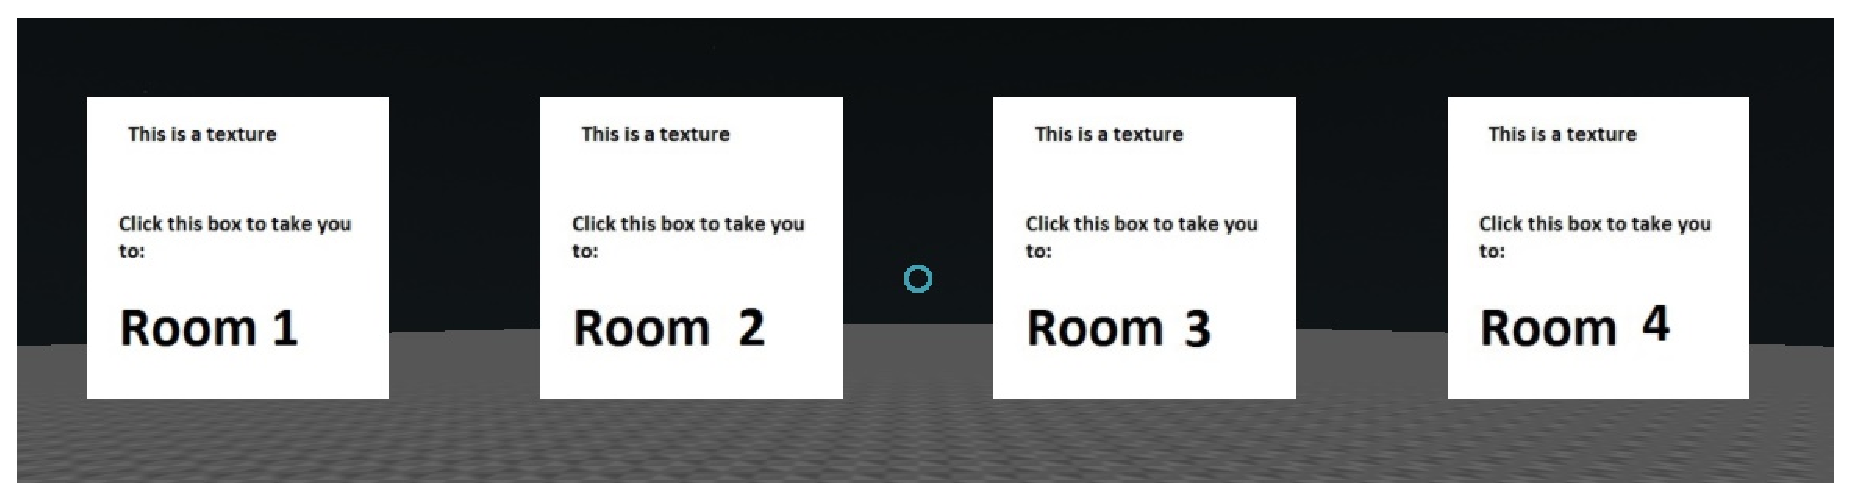
\includegraphics[width=\textwidth]{lobby.eps}\\
%\textbf{Figure 1. } The lobby with eight traversal links to new rooms.\\
%\vspace{.75cm}
%\includegraphics[width=\textwidth]{room1.eps}\\
%\textbf{Figure 2. } Room 1 with multiple trees scattered in the scene.\\
%\vspace{.75cm}
%\includegraphics[width=\textwidth]{room2.eps}\\
%\textbf{Figure 3. } Room 2 demonstrating some animations (it actually is animated).\\
%\vspace{.75cm}
%\includegraphics[width=\textwidth]{room3.eps}\\
%\textbf{Figure 4. } Room 3 has some specific user interactions when hovering over the spheres. \\
%\vspace{.75cm}
%\includegraphics[width=\textwidth]{room4.eps}\\
%\textbf{Figure 5. } Room 4 combines all aspect to put together an interesting scene. \\
%\vspace{.75cm}

%\includegraphics[width=\textwidth]{room1r.eps}\\
%\textbf{Figure 6. } Room 1r with multiple High polygon trees scattered in the scene.\\
%\vspace{.75cm}
%\includegraphics[width=\textwidth]{room2r.eps}\\
%\textbf{Figure 7. } Room 2r demonstrating some animations while loading high textures (it actually is animated).\\
%\vspace{.75cm}
%\includegraphics[width=\textwidth]{room3r.eps}\\
%\textbf{Figure 8. } Room 3r has some specific user interactions when hovering over the spheres. \\
%\vspace{.75cm}
%\includegraphics[width=\textwidth]{room4r.eps}\\
%\textbf{Figure 9. } Room 4r combines all aspect to put together an interesting scene. \\
%\vspace{.75cm}
%\end{center}
\end{singlespace}

\newpage
\begin{thebibliography}{9}



\bibitem{android} 
Vogella. 
\textit{Android Application Performance Profiling through Android SDK}. 
\\\texttt{http://www.vogella.com/tutorials/AndroidTools/article.html}

\bibitem{firefox} 
Mozilla Developer Network.
\textit{Firefox Developer Tools}.
\\\texttt{https://developer.mozilla.org/en-US/docs/Tools}

\bibitem{chrome} 
Google Chrome DevTools. 
\textit{Chrome DevTools}.
\\\texttt{https://developers.google.com/web/tools/chrome-devtools/}

\bibitem{phonespec}
GSM Arena.
\textit{Phone Specifications}
\\\texttt{http://www.gsmarena.com/}

\bibitem{aframe} 
A-Frame. 
\textit{Building a Basic Scene in A-Frame}.
\\\texttt{https://aframe.io/docs/0.2.0/guide/building-a-basic-scene.html}

\end{thebibliography}


\end{document}
